% Settings for the default beamer theme
\documentclass[english, aspectratio=169]{beamer}
\usepackage[T1]{fontenc}
\usepackage[utf8]{inputenc}
\usepackage{tabularx}
\usepackage{babel}
\usepackage[ruled,vlined]{algorithm2e}
\SetAlgorithmName{Algoritmus}{algoritmus}{List of Algorithms}
\setcounter{secnumdepth}{3}
\setcounter{tocdepth}{3}

\makeatletter

\newcommand\makebeamertitle{\frame{\maketitle}}

% (ERT) argument for the TOC
\AtBeginDocument{%
  \let\origtableofcontents=\tableofcontents
  \def\tableofcontents{\@ifnextchar[{\origtableofcontents}{\gobbletableofcontents}}
  \def\gobbletableofcontents#1{\origtableofcontents}
}

% Theme settings
\usetheme{Frankfurt}
\usecolortheme{default}
\usefonttheme[onlymath]{serif}

% Template settings
\setbeamertemplate{navigation symbols}{}
\setbeamertemplate{blocks}[rounded][shadow=false]
\setbeamertemplate{title page}[default][colsep=-4bp, rounded=true, shadow=false]
\makeatother

% Define a custom darker red color
\definecolor{DarkerRed}{RGB}{139,0,0} % Adjust the RGB values as needed

% Use the newly defined color in Beamer theme elements
\setbeamercolor{structure}{fg=DarkerRed} % Changes basic structural elements to Darker Red
\setbeamercolor{title in head/foot}{bg=DarkerRed} % Changes the title in header/footer to Darker Red


\begin{document}

% Title page
\section{Dimenzionalitás}
\title[]{Üzleti Elemzések Módszertana}
\subtitle{7. Előadás: Felügyelet nélküli tanulás}
\author[Kuknyó Dániel]{Kuknyó Dániel\\Budapesti Gazdasági Egyetem}
\date{2023/24\\2.félév}
\makebeamertitle

% Table of contents slide
\begin{frame}
\tableofcontents{}
\end{frame}

% Table of contents of the current section
\begin{frame}
\tableofcontents[currentsection]
\end{frame}

\begin{frame}{A dimenzionalitás átka}
Az érzékek \textbf{gyakran megcsalhatják az embereket, mert 3D-be vannak zárva}. A matematikában viszont lehetséges számolni magasabb dimenziókkal. Sok koncepció \textbf{nagyon különbözően viselkedik magasabb dimenzióban mint alacsonyabban}.\par\smallskip
Például: egy egység négyzetben az a valószínűség, hogy egy véletlen pont 0.001-nél közelebb lesz egy élhez, 0.4\%. Ugyanez a valószínűség egy 10000 dimenziós hiperkocka esetén 99.99999\%.
\begin{center}
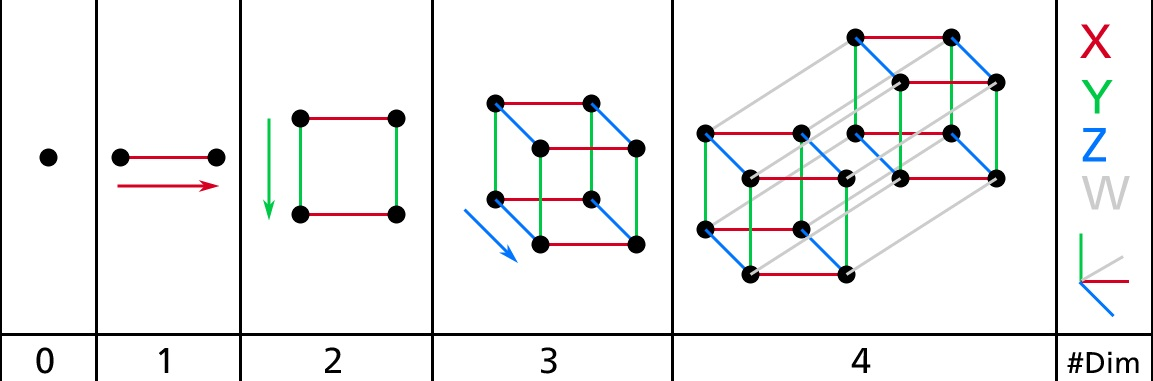
\includegraphics[width=10cm, keepaspectratio]{images/unsupervised_1.png}
\end{center}
\end{frame}

\begin{frame}{Dimenziócsökkentés}
Olyan eljárások, amelyek \textbf{egy magasabb dimenziós térből egy alacsonyabb dimenziós térbe transzformálják az adatokat} amellett, hogy a fontos információtartalom ne vesszen el. Főbb eljárásai a jellemzőkiválasztás, jellemző összevonás, manifold tanulás, izometrikus leképezés.\par\medskip
\begin{center}
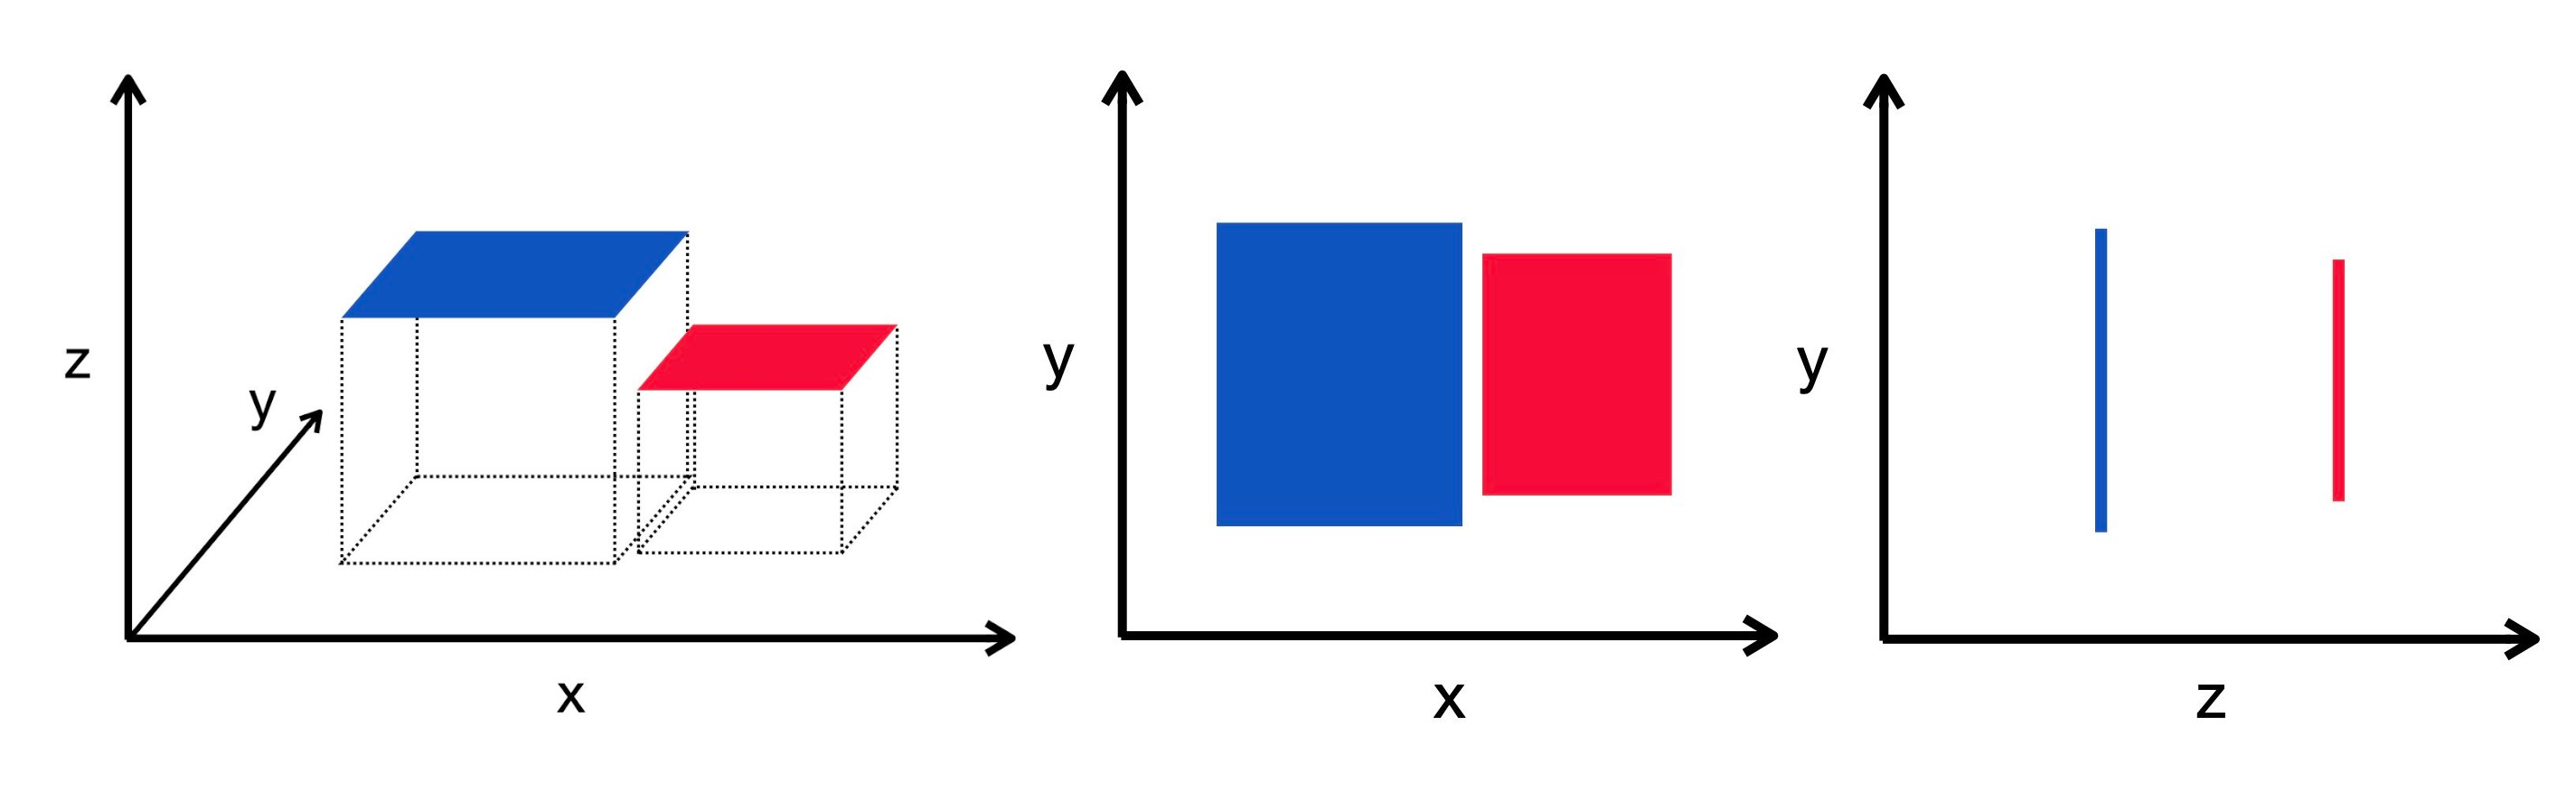
\includegraphics[width=12cm, height=7cm, keepaspectratio]{images/unsupervised_2.png}
\end{center}
\end{frame}

\section{Manifold tanulás}

\begin{frame}
\tableofcontents[currentsection]
\end{frame}

\begin{frame}{Projekció}
\begin{columns}
\begin{column}{.5\textwidth}
A projekció, mint dimenziócsökkentési eljárás, egy adathalmaz tulajdonságainak vagy jellemzőinek csökkentett dimenziójú térbe való leképezését jelenti.
\begin{center}
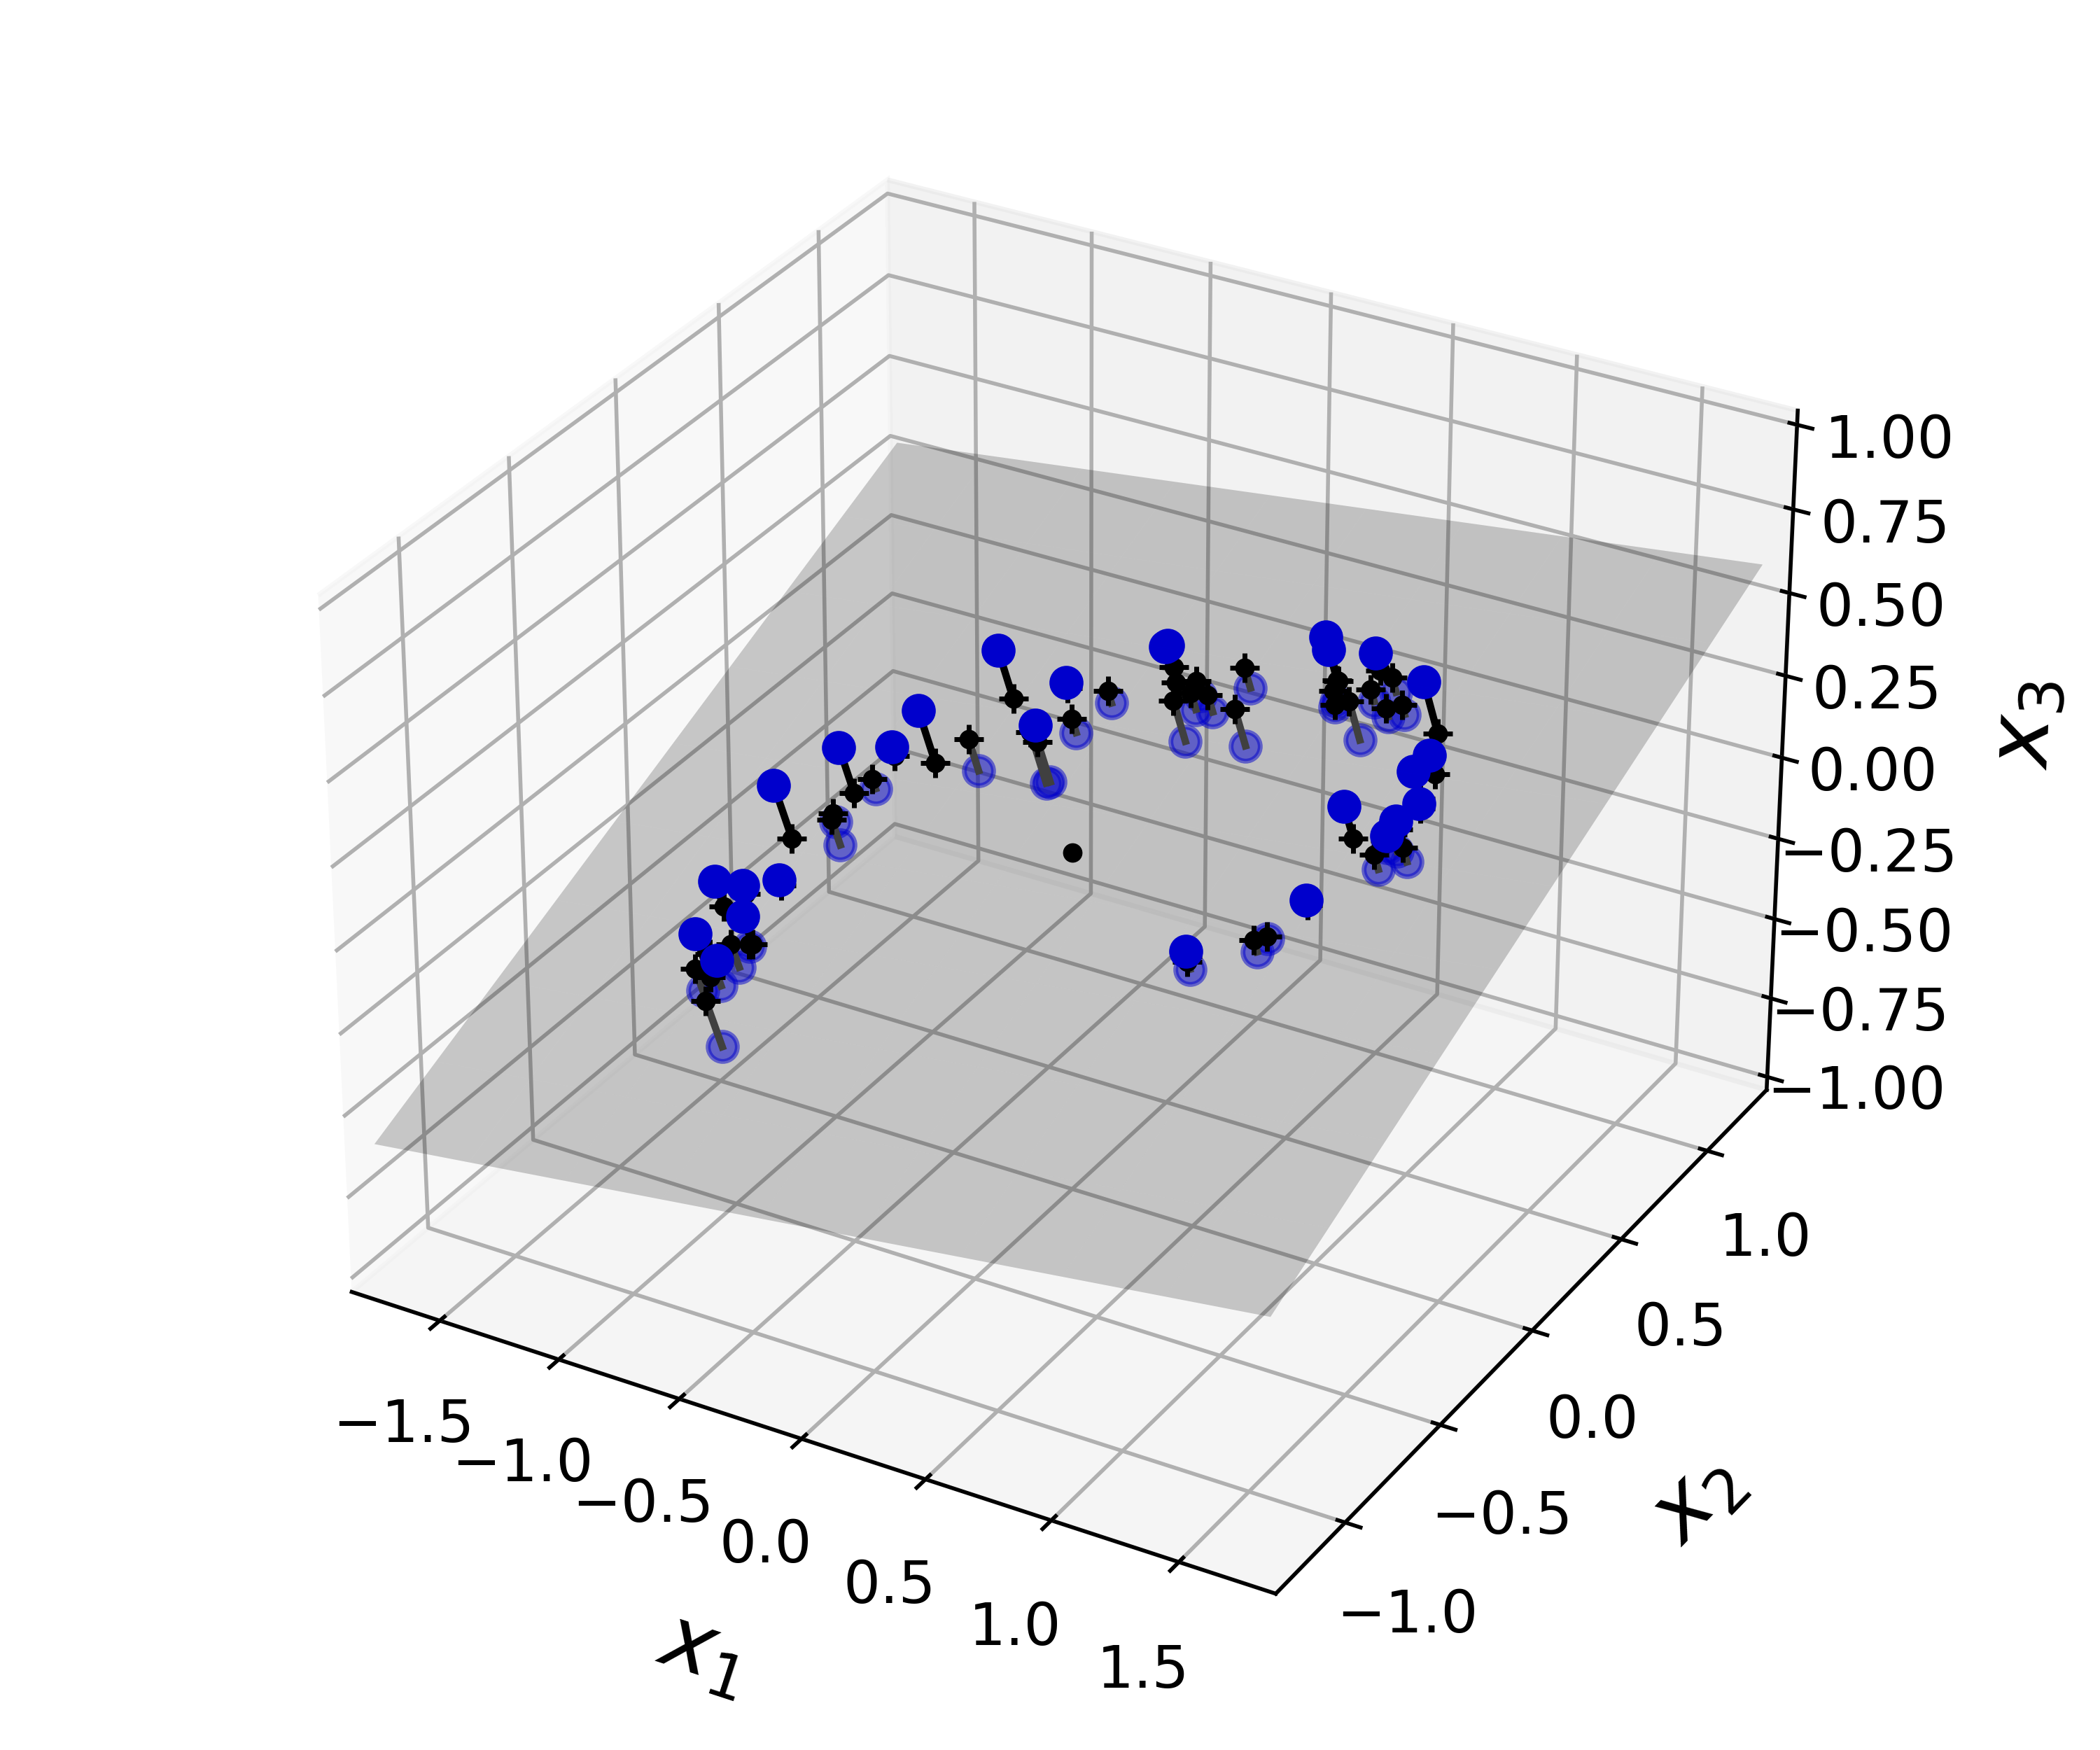
\includegraphics[width=6cm, keepaspectratio]{images/unsupervised_3.png}
\end{center}
\end{column}
\begin{column}{.5\textwidth}
Ez a folyamat lehetővé teszi, hogy a magas dimenziójú adatok egyszerűbb, kezelhetőbb formában való vizsgálatát. 
\begin{center}
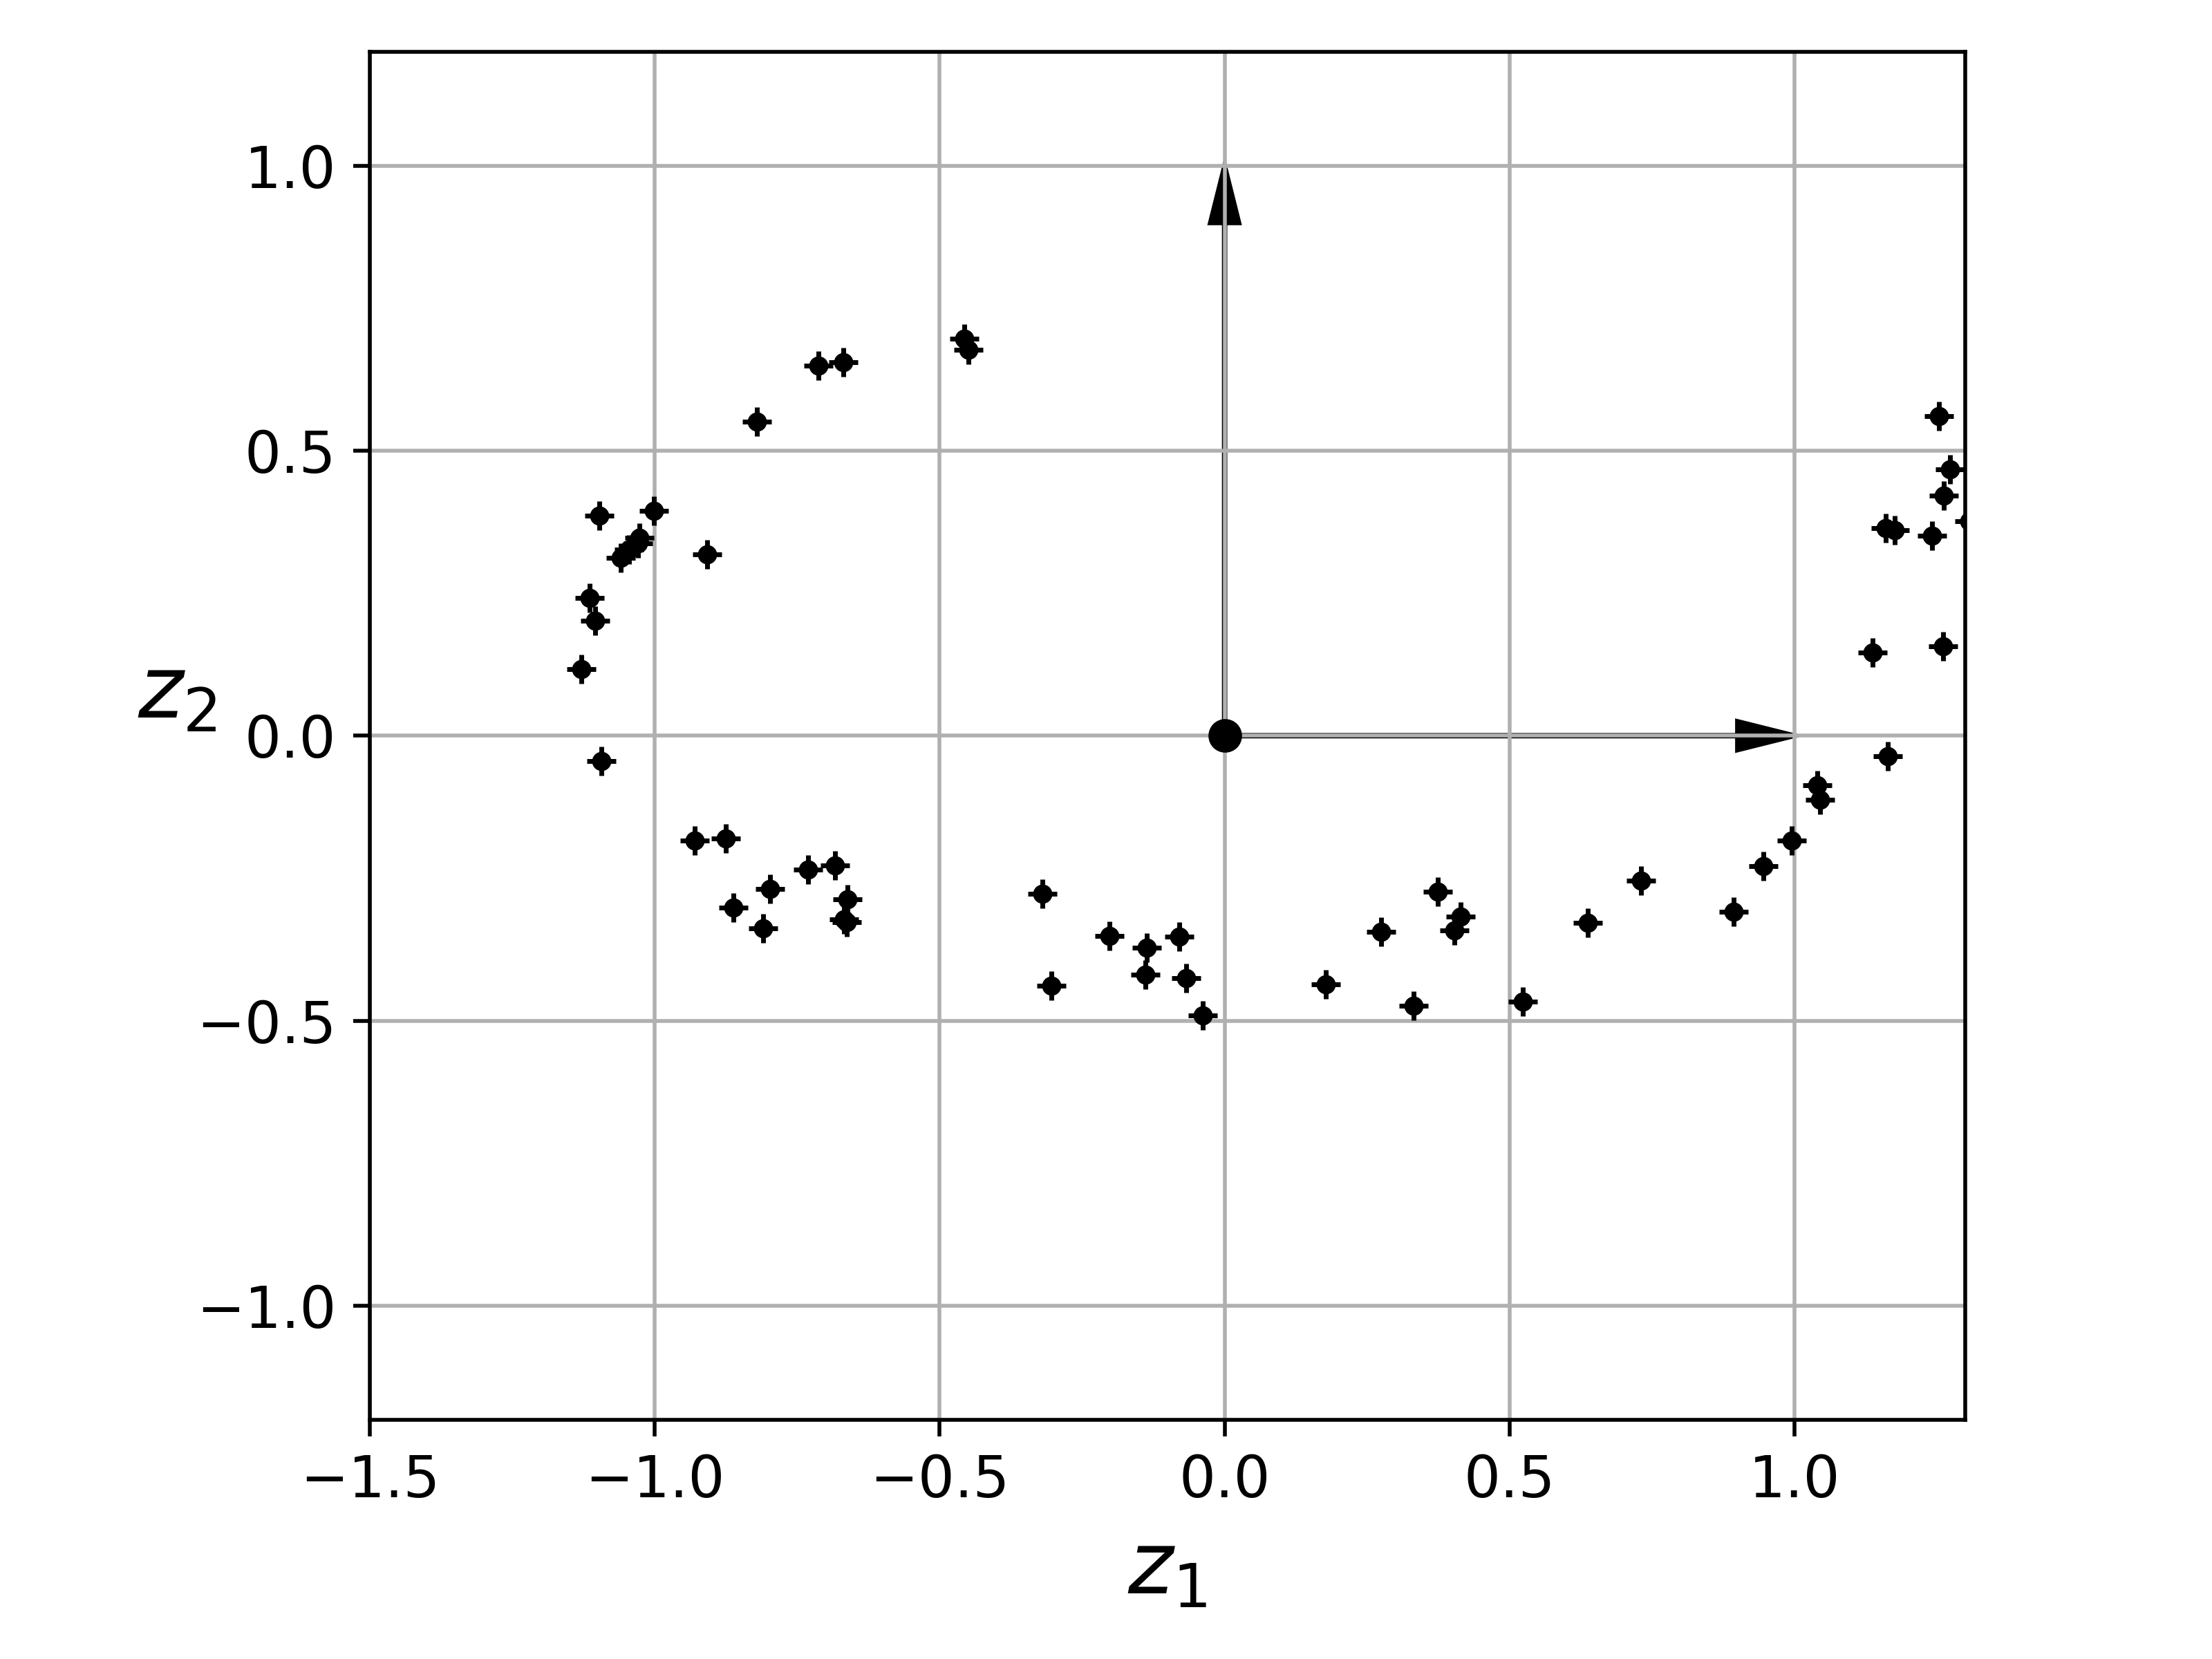
\includegraphics[width=6cm, keepaspectratio]{images/unsupervised_4.png}
\end{center}
\end{column}
\end{columns}
\end{frame}

\begin{frame}{A svéd tekercs}
\begin{columns}
\begin{column}{.5\textwidth}
A svéd tekercs egy gyakran használt tesztelő adathalmaz a manifold tanulás területén.\par\smallskip
A manifold tanulás célja \textbf{a magas dimenziós adatok alacsony dimenziós, de topologikusan hű reprezentációjának megtalálása}. A svéd tekercs egy 3D-ben lévő 2D-s manifold, amely két dimenzióban van tekerve vagy spirálozva.\par\medskip
A feladat a tekercs lehajtása a belső struktúrájának megőrzésével.
\end{column}
\begin{column}{.5\textwidth}
\begin{center}
\includegraphics<1>[width=7cm, keepaspectratio]{images/unsupervised_5.png}
\includegraphics<2>[width=7cm, keepaspectratio]{images/unsupervised_6.png}
\includegraphics<3>[width=7cm, keepaspectratio]{images/unsupervised_7.png}
\end{center}
\end{column}
\end{columns}
\end{frame}

\begin{frame}{A manifold hipotézis}
\begin{columns}
\begin{column}{.5\textwidth}
\begin{block}{Manifold hipotézis}
A manifold feltevés két alapvetően fontos dolgot állít:
\begin{itemize}
	\item Az adathalmazban \textbf{rejlenek} manifoldok. Ez leggyakrabban empírikusan megfigyelhető.
	\item A feladat \textbf{könnyebb lesz}, ha a manifoldnak egy alacsonyabb dimenziós terében próbáljuk megoldani.
\end{itemize}
\end{block}
A manifold tanulás nem minden esetben alkalmazható.
\end{column}
\begin{column}{.5\textwidth}
\begin{center}
\includegraphics<1>[width=7cm, keepaspectratio]{images/unsupervised_8.png}
\includegraphics<2>[width=7cm, keepaspectratio]{images/unsupervised_9.png}
\includegraphics<3>[width=7cm, keepaspectratio]{images/unsupervised_10.png}
\includegraphics<4>[width=7cm, keepaspectratio]{images/unsupervised_11.png}
\end{center}
\end{column}
\end{columns}
\end{frame}

\section{Dimenziócsökkentés}

\begin{frame}
\tableofcontents[currentsection]
\end{frame}

\begin{frame}{Főkomponenselemzés}
Az egyik legnépszerűbb dimenziócsökkentő algoritmus. Először felfedezi azt a hipersíkot, amely a legközelebb van az adatokhoz, majd ráprojektálja az adatpontokat.\par\smallskip
Az eljárás maximalizálja az eredeti adathalmaz és a projekciója közötti varianciát, hiszen az információ a varianciában rejlik.
\begin{center}
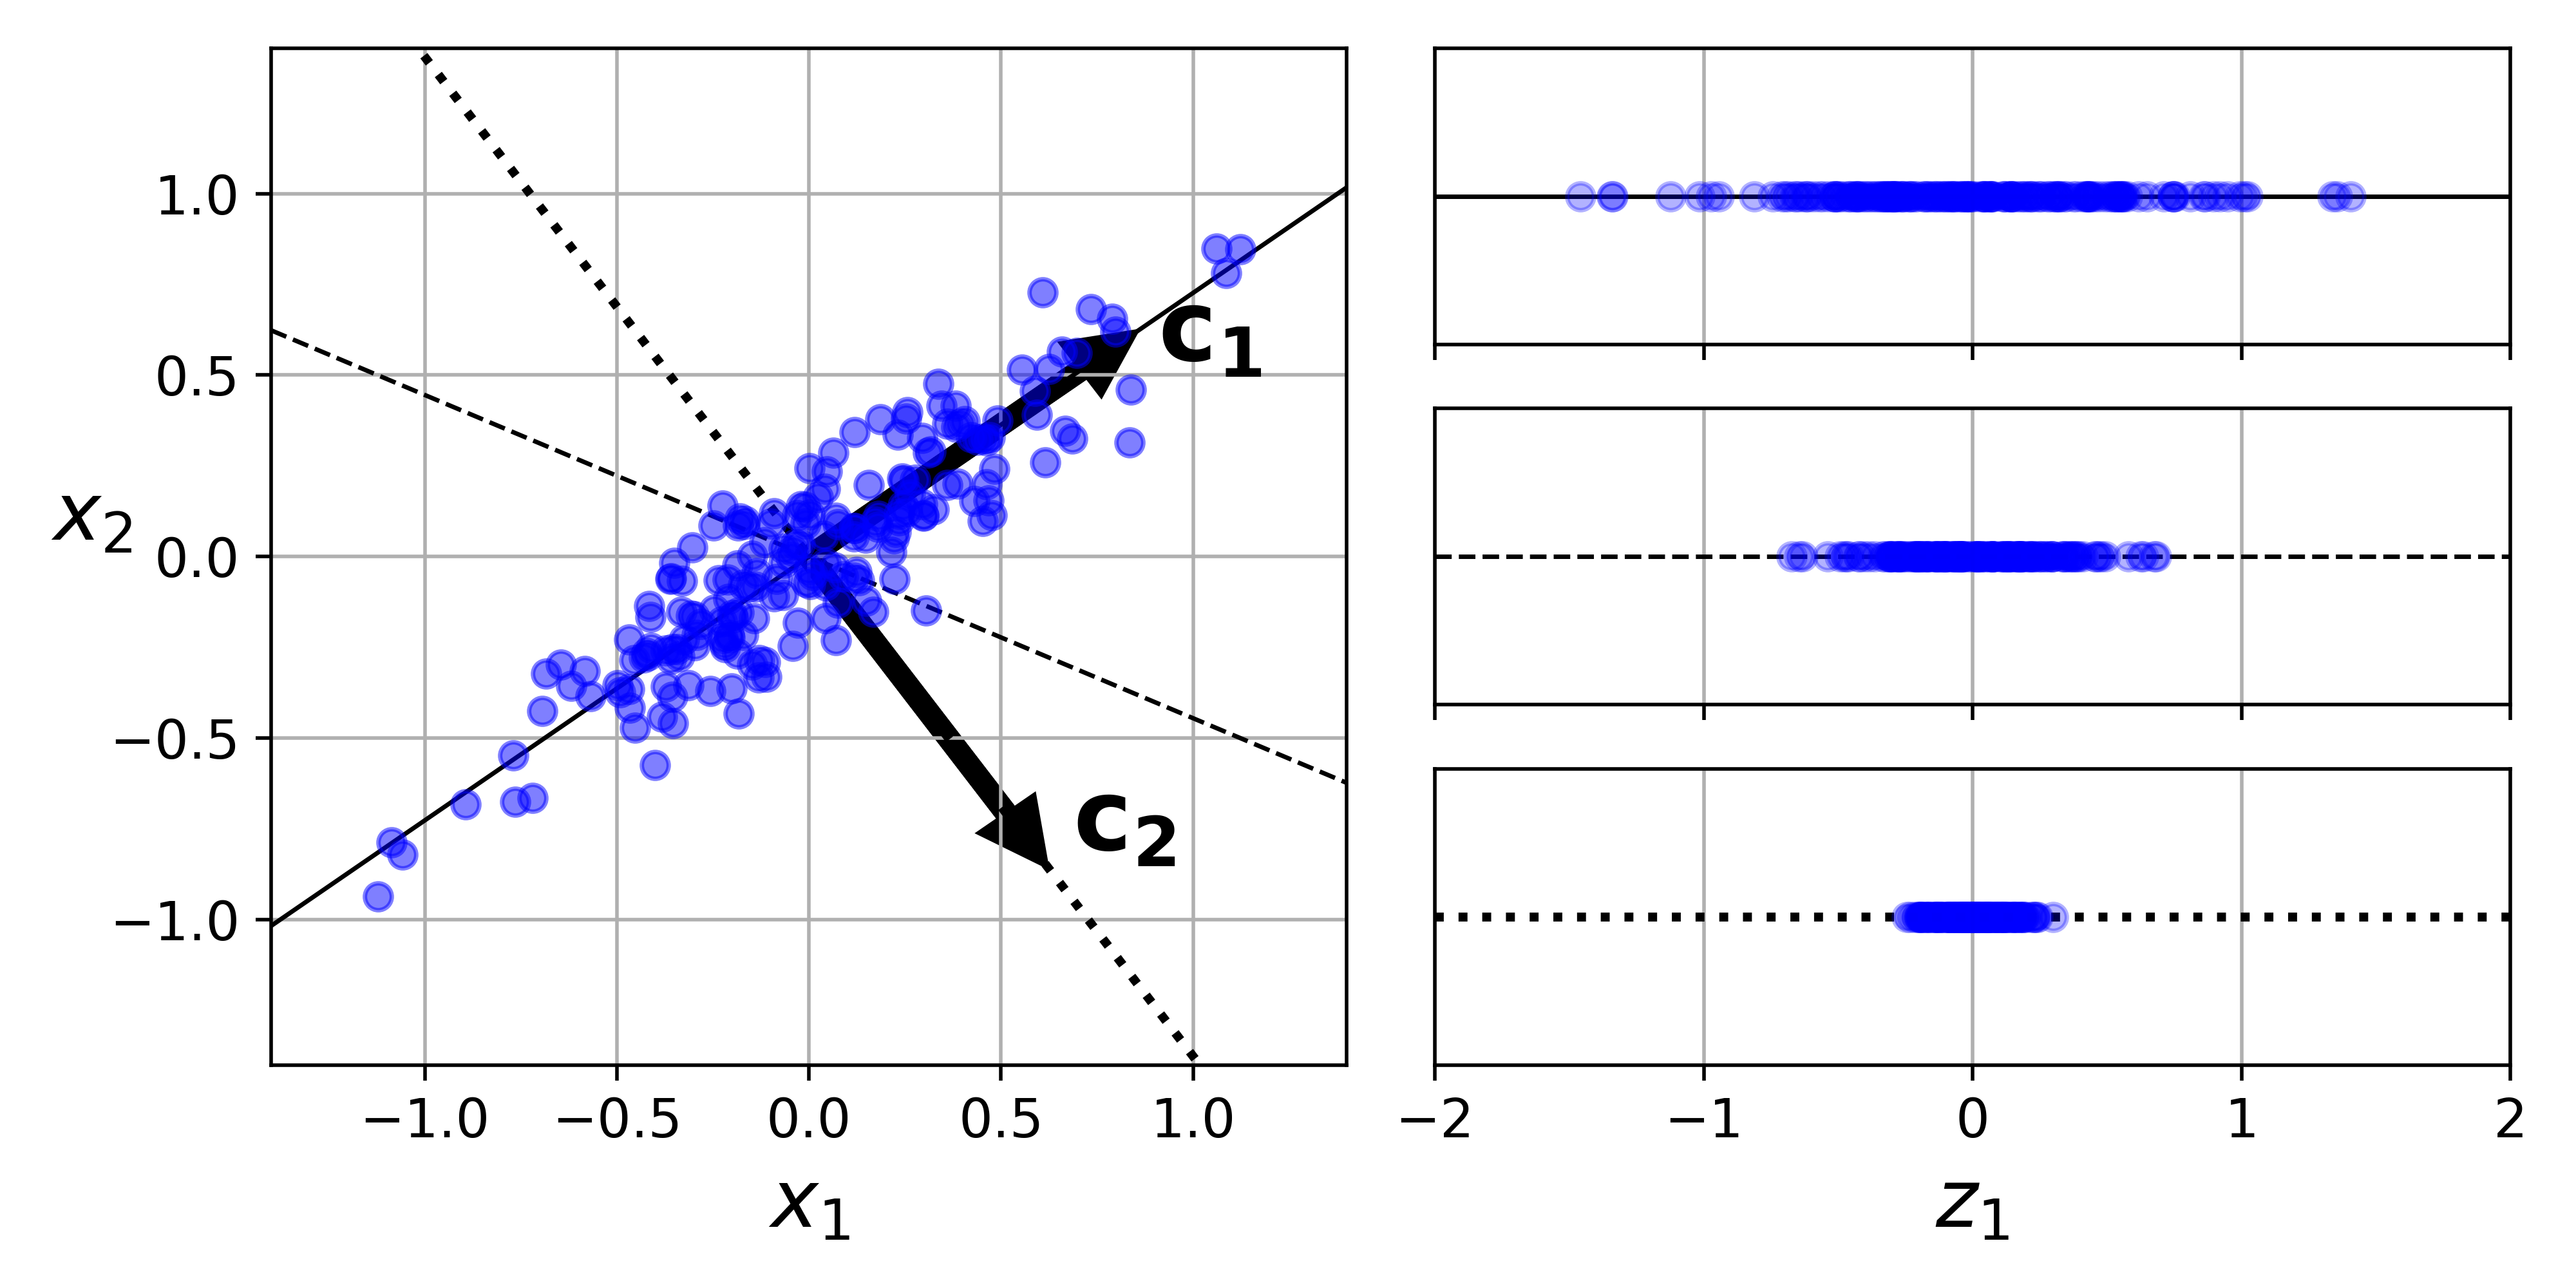
\includegraphics[width=10cm, keepaspectratio]{images/unsupervised_12.png}
\end{center}
\end{frame}

\begin{frame}{Szinguláris értékfelbontás}
\begin{columns}
\begin{column}{.6\textwidth}
\begin{block}{Szinguláris értékfelbontás}
Legyen az egységvektor, amelyik az $i$-edik tengelyt definiálja, az $i$-edik főkomponens: $c_1, c_2, \ldots, c_n$.\par\smallskip
Az eljárás $M\in \mathbb{R}$ mátrixot három mátrixra bontja $M = U \Sigma V^T$:
\begin{itemize}
	\item $U$: $n$ db ortonormált sajátvektort tartalmaz
	\item $\Sigma$: Főátlóján találhatóak a szinguláris értékek
	\item $V$: A keresett főkomponenseket tartalmazza
\end{itemize}
A főkomponensek létrejötte után a projekcióhoz $M$ tanító adathalmaz mátrix és $W_d$ főkomponenseket tartalmazó mátrix szorzatát kell képezni: $M_{d-proj} = M \cdot W_d$.
\end{block}
\end{column}
\begin{column}{.4\textwidth}
\begin{center}
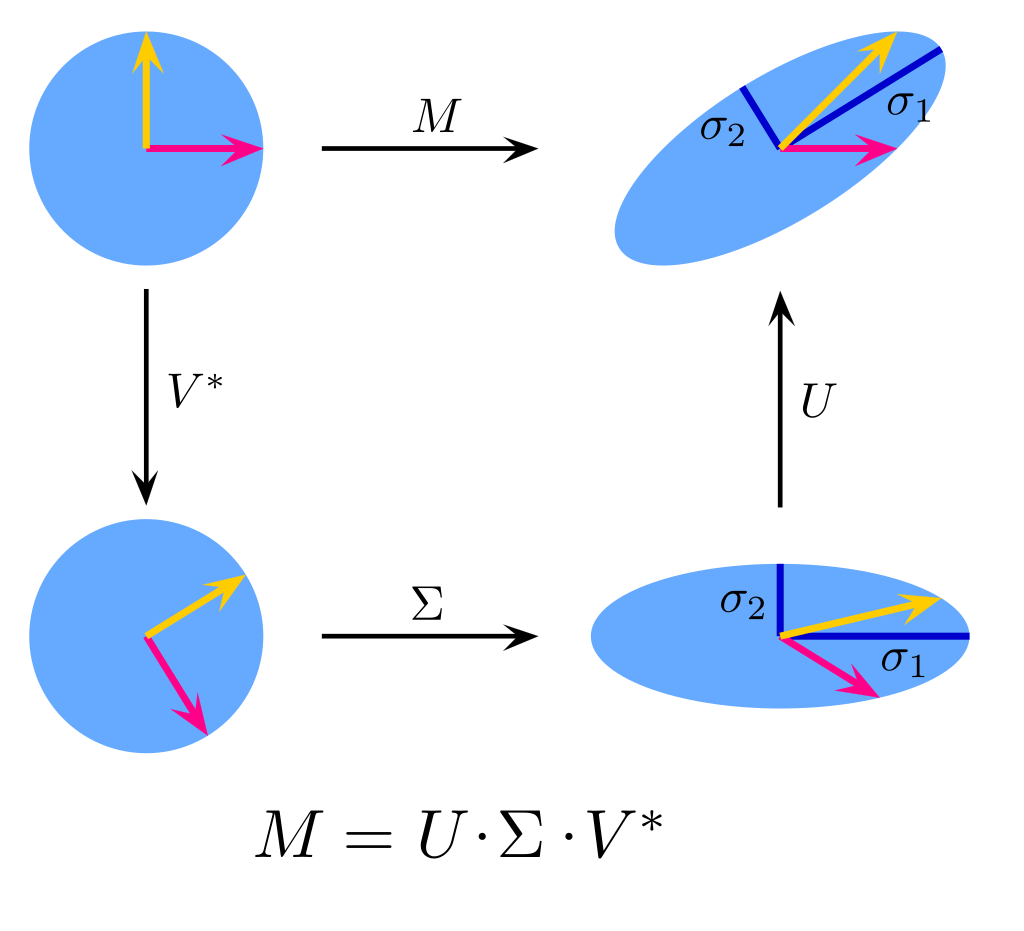
\includegraphics[width=6cm, height=7cm, keepaspectratio]{images/unsupervised_13.png}
\end{center}
\end{column}
\end{columns}
\end{frame}

\begin{frame}{A megfelelő dimenziószám kiválasztása}
\begin{columns}
\begin{column}{.5\textwidth}
\only<1>{A dimenziók száma a PCA hiperparamétere, ezért létrejöttek eljárások a finomhangolására. Az egyik ilyen eljárás a könyök módszer:\par\smallskip
A könyök módszer szerint ahol \textbf{elkezd csökkenni a modell által megmagyarázott variancia} növekedési üteme, ott könyökpont található, nem kell több dimenziót bevonni a modellezésbe.}
\only<2>{\begin{block}{Megmagyarázott varianciahányad}
Megadja, hogy az egyes főkomponensek, vagy dimenziók, \textbf{milyen mértékben járulnak hozzá az eredeti adathalmaz varianciájának magyarázatához}.\par\medskip
A főkomponensek varianciájának és az összes varianciának a hányadosa.
\end{block}}
\end{column}
\begin{column}{.5\textwidth}
\begin{center}
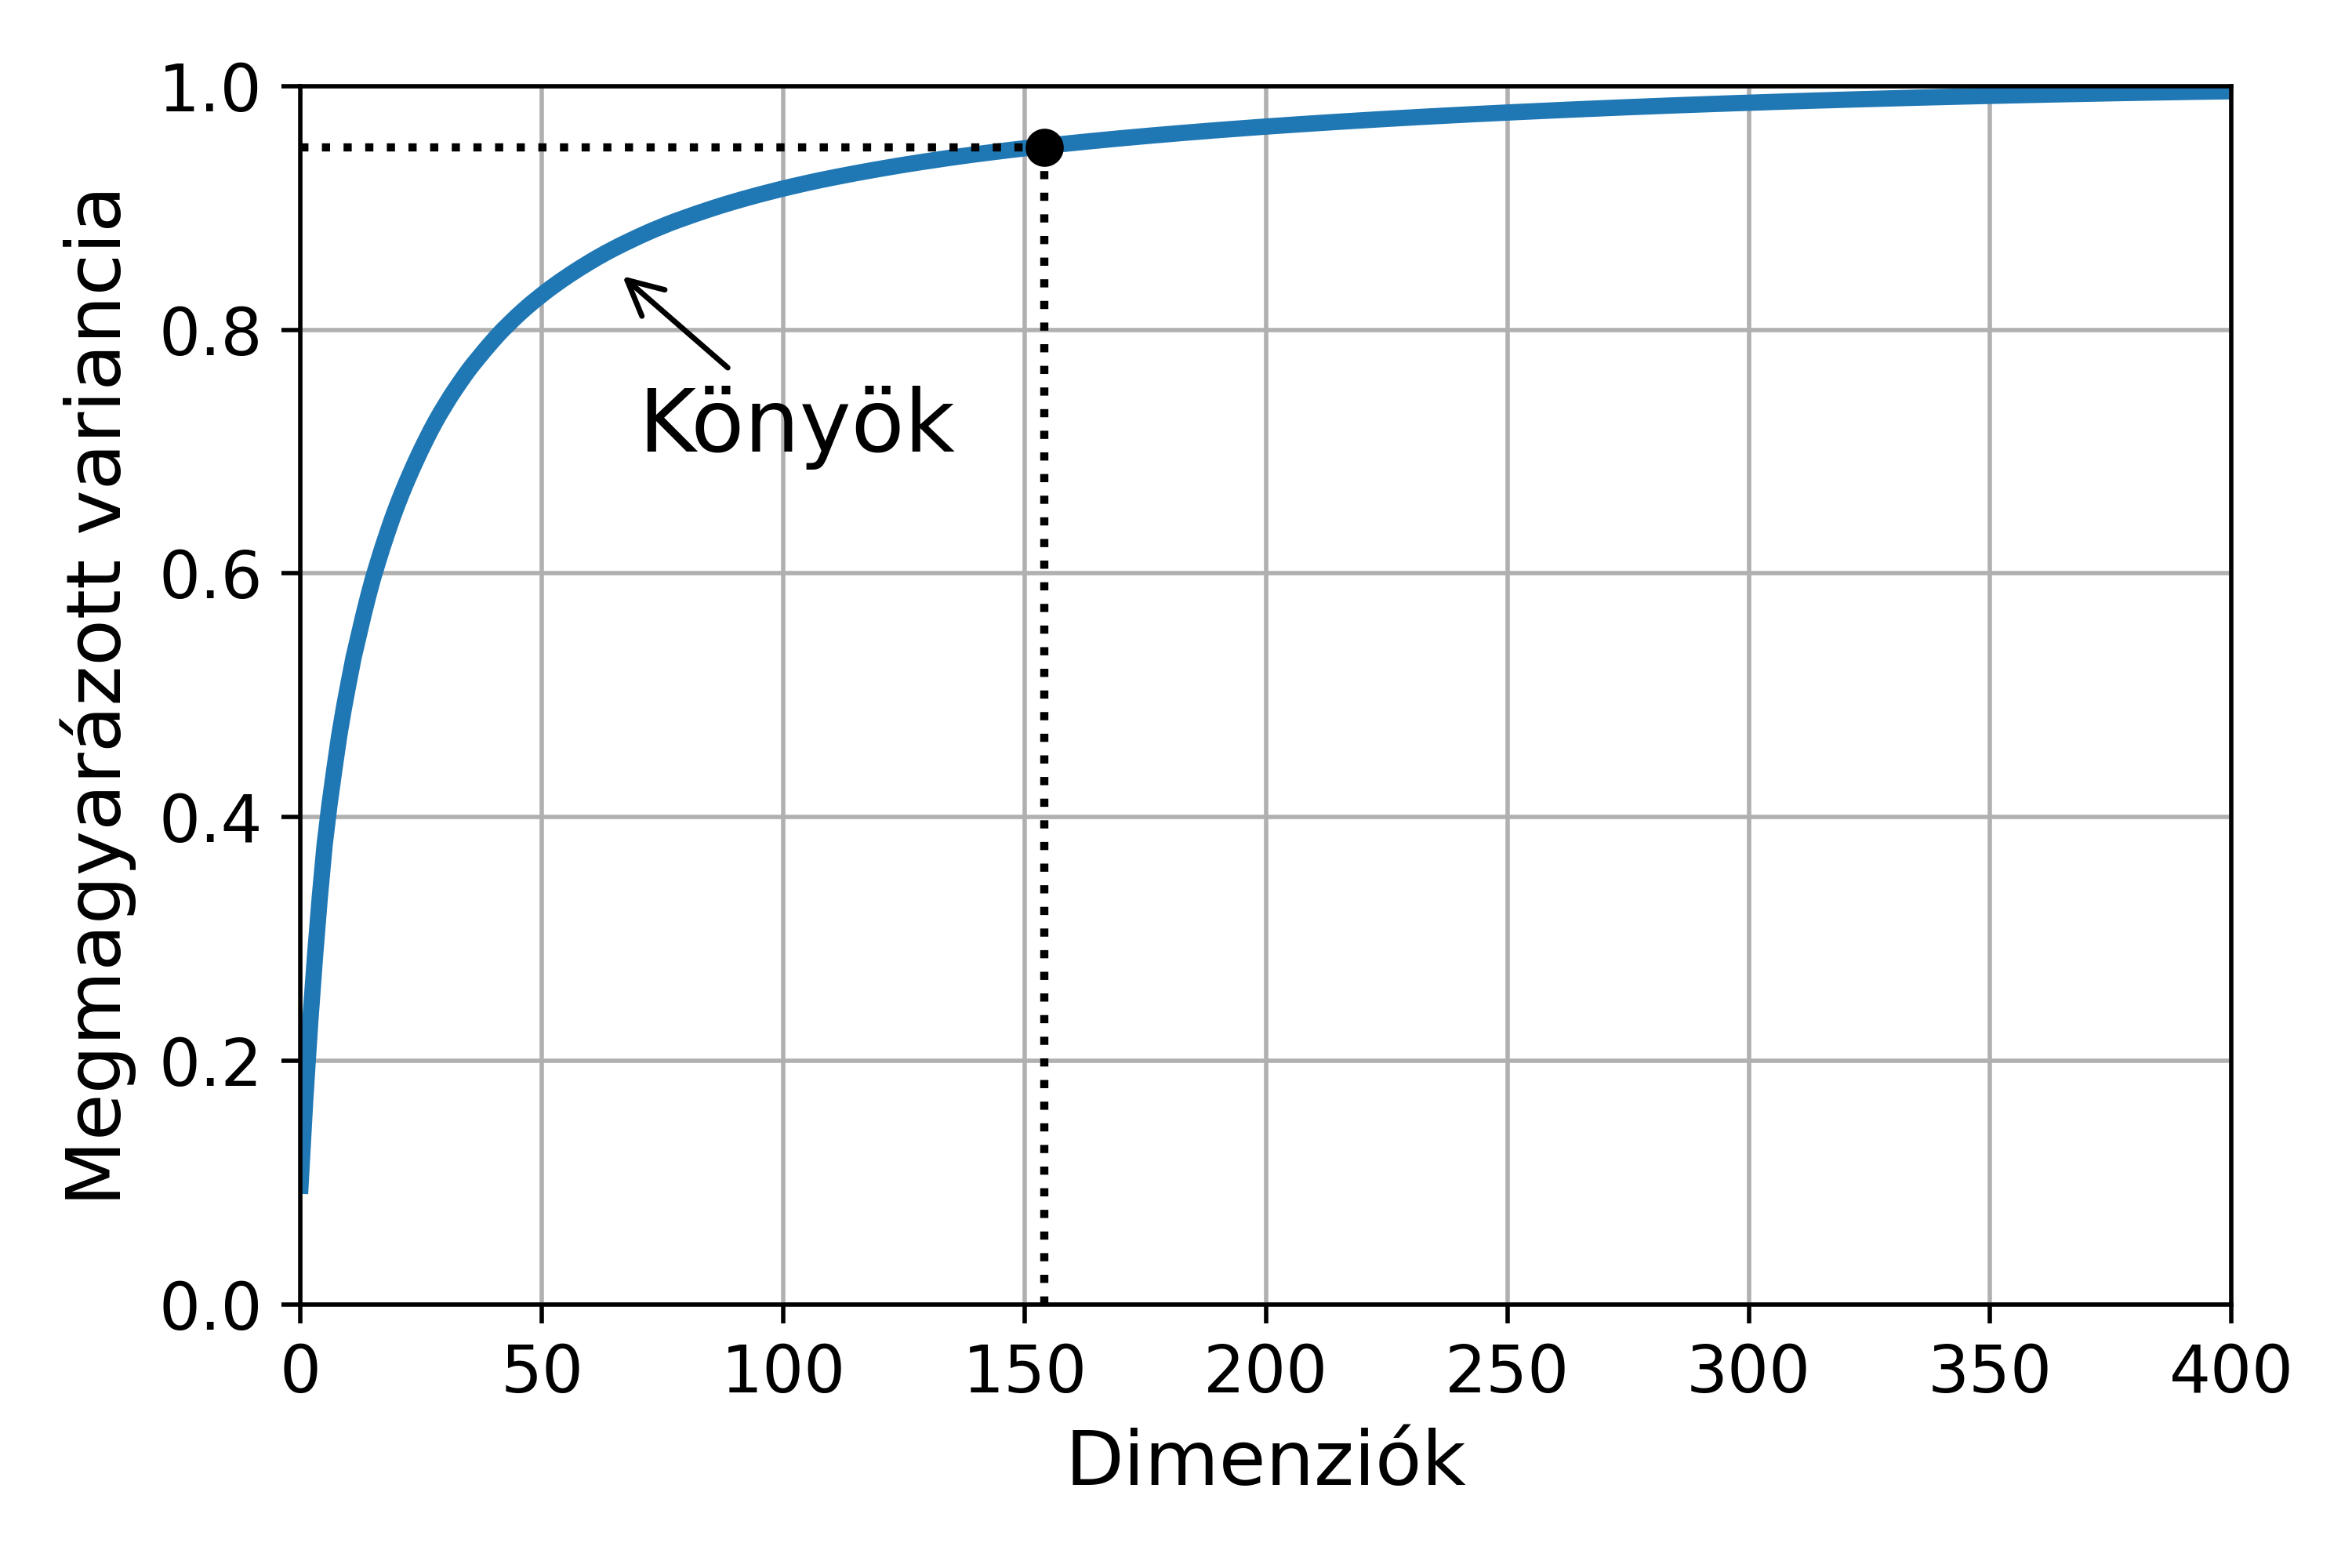
\includegraphics[width=7cm, height=7cm, keepaspectratio]{images/unsupervised_14.png}
\end{center}
\end{column}
\end{columns}
\end{frame}

\begin{frame}{PCA, mint tömörítési eljárás}
\begin{columns}
\begin{column}{.5\textwidth}
Dimenziócsökkentés után az adatkészlet kevesebb memóriát foglal.\par\smallskip
Az MNIST adathalmazban 95\% variancia megtartással 28x28 képek esetén 784 jellemzőből 150 maradt. Ez több, mint 80\% csökkenés 5\% varianciáért cserébe.\par\smallskip
A transzformáció fordított irányba is lehetséges:
\begin{block}{}
\vspace{-.2cm}
\[
X_{recovered} = X_{d-proj} W_d^T
\]
\end{block}
\end{column}
\begin{column}{.5\textwidth}
\begin{center}
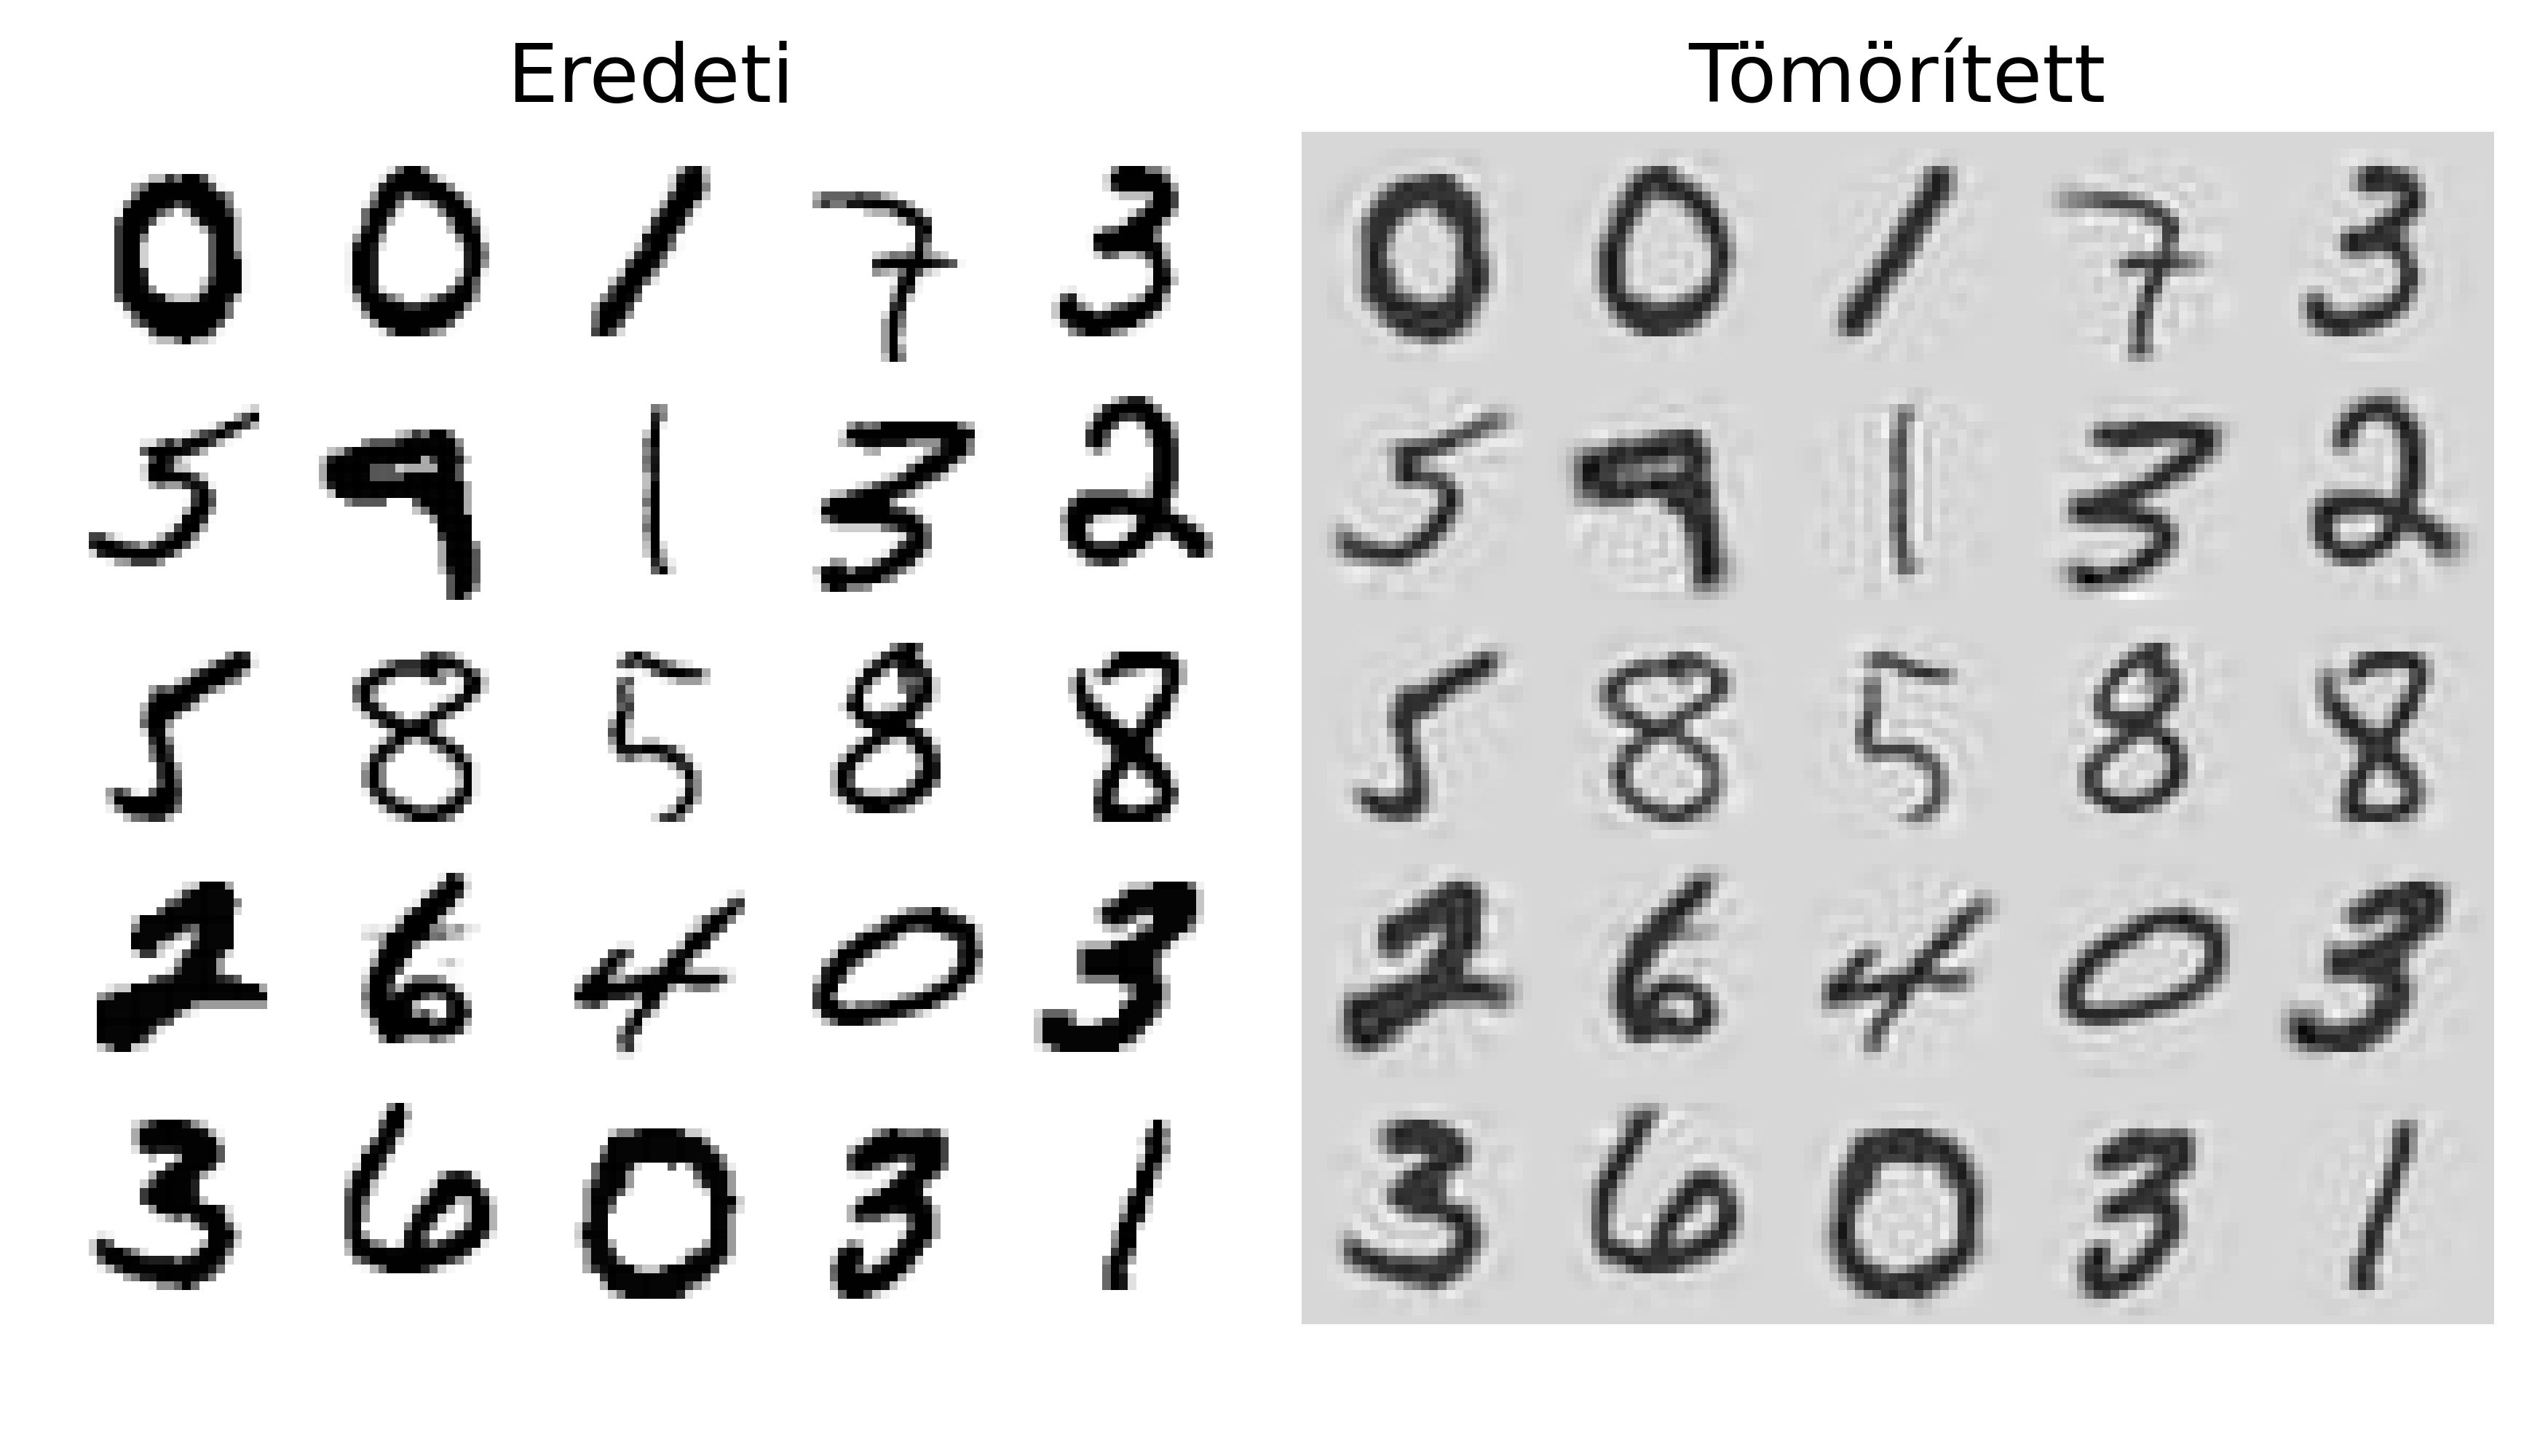
\includegraphics[width=7cm, height=7cm, keepaspectratio]{images/unsupervised_15.png}
\end{center}
\end{column}
\end{columns}
\end{frame}

\begin{frame}{Dimenziócsökkentés az MNIST adatokon}
\begin{columns}
\begin{column}{.5\textwidth}
A képen az MNIST adathalmaz látható T-SNE (T-eloszlású sztochasztikus szomszéd beágyazás) modell által 2 dimenzióba projektálva.\par\smallskip
\end{column}
\begin{column}{.5\textwidth}
\begin{center}
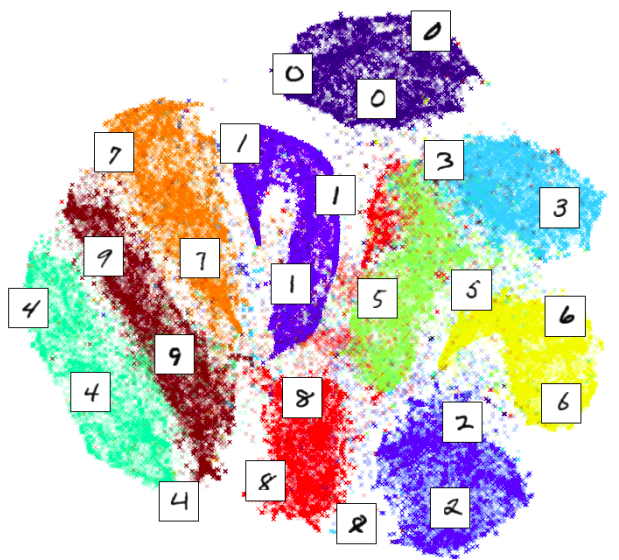
\includegraphics[width=6cm, height=7cm, keepaspectratio]{images/unsupervised_16.png}
\end{center}
\end{column}
\end{columns}
\end{frame}

\section{Klaszteranalízis}

\begin{frame}
\tableofcontents[currentsection]
\end{frame}

\begin{frame}{Klaszteranalízis}
\begin{columns}
\begin{column}{.5\textwidth}
A klaszteranalízis feladata \textbf{felismerni az egymással hasonló egyedeket, majd csoportokba (klaszterekbe) rendezni őket}.\par\smallskip
A klaszterezés egy \textbf{felügyelet nélküli tanulási módszer}, tehát az adatok címkéi nem ismertek a tanítási folyamat során, a modell feladata ezeket megtalálni.
Főbb felhasználásai:
\begin{itemize}
	\item Vásárló szegmentálás
	\item Új adatok elemzése
	\item Dimenziócsökkentés
	\item Anomália detekció
	\item Képek szegmentálása
\end{itemize}
\end{column}
\begin{column}{.5\textwidth}
\begin{center}
\includegraphics<1>[width=7cm, height=7cm, keepaspectratio]{images/unsupervised_17}
\includegraphics<2>[width=7cm, height=7cm, keepaspectratio]{images/unsupervised_18}
\includegraphics<3>[width=7cm, height=7cm, keepaspectratio]{images/unsupervised_19}
\end{center}
\end{column}
\end{columns}
\end{frame}

\begin{frame}{A $K$-közép algoritmus}
\begin{columns}
\begin{column}{.5\textwidth}
A $K$ közép algoritmus célja megkeresni minden csoport középpontját, majd minden adatpontot a hozzá legközelebb eső középponthoz rendel. Ez a középpont a \textbf{centroid}.\par\smallskip
A létrehozandó klaszterek száma $K$ az algoritmus hiperparamétere, tehát a tanítónak kell megadnia a futtatás előtt.\par\smallskip
A létrejövő döntési határok egy \textbf{Voronoi-tesszellációt} határoznak meg. 
\end{column}
\begin{column}{.5\textwidth}
\begin{center}
\includegraphics<1>[width=7cm, height=7cm, keepaspectratio]{images/unsupervised_20}
\includegraphics<2>[width=7cm, height=7cm, keepaspectratio]{images/unsupervised_21}
\end{center}
\end{column}
\end{columns}
\end{frame}

\begin{frame}{A $K$-közép működése}
\begin{columns}
\begin{column}{.5\textwidth}
Az algoritmus két lépést ismétel, ameddig a klaszter centroidok mozgása nem lassul le a kilépési határ alá: 
\begin{enumerate}
	\item Véletlenszerű centroid inicializáció
	\item Minden egyed hozzárendelése a hozzá legközelebb eső centroidhoz
	\item Minden centroid mozgatása a hozzá tartozó egyedek várható értékére
\end{enumerate}
\end{column}
\begin{column}{.5\textwidth}
\begin{center}
\includegraphics<1>[width=7cm, keepaspectratio]{images/unsupervised_22.png}
\includegraphics<2>[width=7cm, keepaspectratio]{images/unsupervised_23.png}
\includegraphics<3>[width=7cm, keepaspectratio]{images/unsupervised_24.png}
\includegraphics<4>[width=7cm, keepaspectratio]{images/unsupervised_25.png}
\includegraphics<5>[width=7cm, keepaspectratio]{images/unsupervised_26.png}
\includegraphics<6>[width=7cm, keepaspectratio]{images/unsupervised_27.png}
\end{center}
\end{column}
\end{columns}
\end{frame}

\begin{frame}{Optimális klaszterszám megtalálása}
\begin{columns}
\begin{column}{.5\textwidth}
A korábbi példában $K=5$ volt a klaszterszám, mert ez az adatokra ránézve nyilvánvaló volt. Viszont ez a gyakorlatban nem ennyire nyilvánvaló.\par\smallskip
\textbf{Ha az lenne a cél, hogy a legkevesebb legyen a távolság a centroidok és a pontok között, minden pont centroid lenne}, és $0$ lenne az eltérés.
\begin{block}{Inercia}
A centroidok és a centroidokhoz rendelt pontok távolságainak négyzetösszege. Ahogy $K$ emelkedik, az inercia csökken. 
\end{block}
\end{column}
\begin{column}{.5\textwidth}
\begin{center}
\includegraphics<1>[width=7cm, height=7cm, keepaspectratio]{images/unsupervised_35.png}
\includegraphics<2>[width=7cm, height=7cm, keepaspectratio]{images/unsupervised_36.png}
\end{center}
\end{column}
\end{columns}
\end{frame}

\begin{frame}{A könyök módszer}
\begin{columns}
\begin{column}{.5\textwidth}
Heurisztikus, vizuális technika a klaszterszám meghatározására.\par\smallskip
Az eljárás $K=2$ klaszterszámtól indulva különböző $K$ értékekhez ábrázolja a klaszterkonfiguráció inerciáját.\par\smallskip
\textbf{A könyökpont ott található, ahol az inercia egy jelentős esése után a csökkenés üteme lelassul}. Az optimális klaszterszám a könyökponthoz tartozó $K$ érték.\par\medskip
Hátránya, hogy valamikor nincs könyökpont és valamikor több van. 
\end{column}
\begin{column}{.5\textwidth}
\begin{center}
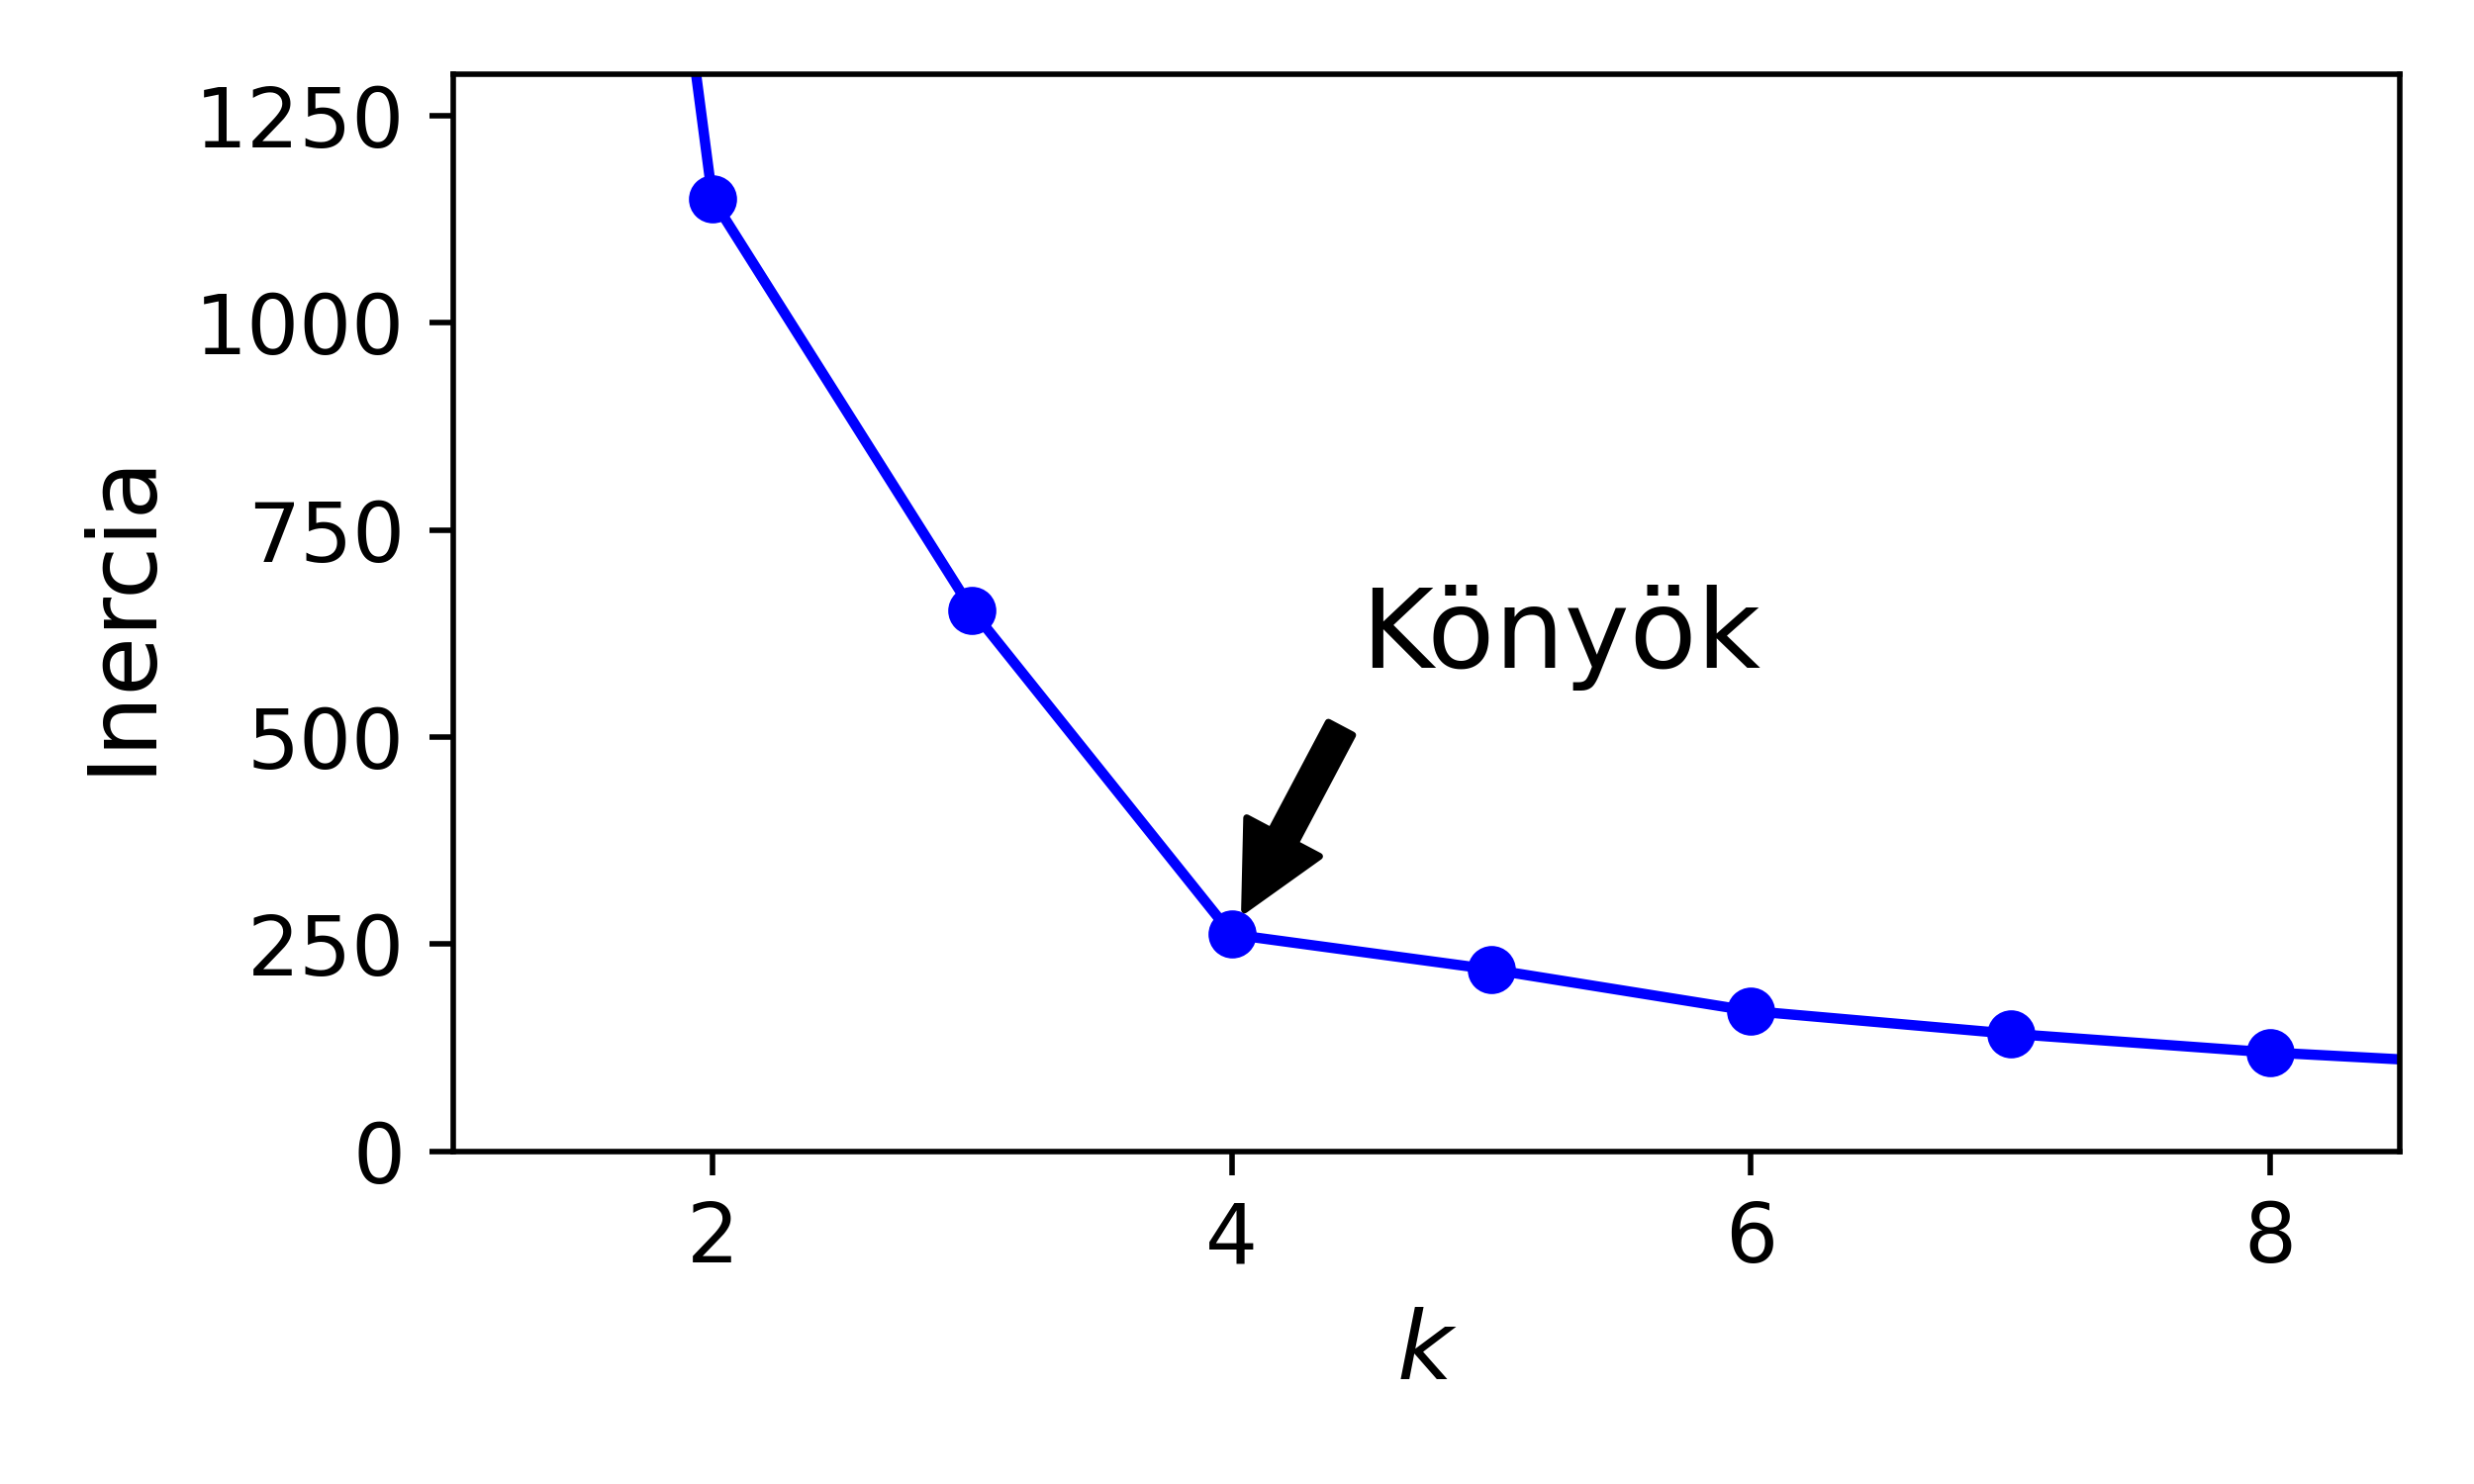
\includegraphics[width=7cm, height=7cm, keepaspectratio]{images/unsupervised_30.png}
\end{center}
\end{column}
\end{columns}
\end{frame}

\begin{frame}{A sziluett együttható}
\begin{columns}
\begin{column}{.5\textwidth}
A sziluett alapja a klaszteren belüli szorosság és a többi egyedtől való távolság tartás mértéke.\par\smallskip
\begin{block}{Sziluett}
Minden $i \in I$ mintaegyedre a sziluett $s\left( i \right)$:
\vspace{-.2cm}
\[
s\left( i \right) = \frac{b\left( i \right) - a\left( i \right)}{max\left( b\left( i \right), a\left( i \right) \right)}
\]
\vspace{-.4cm}
\begin{itemize}
	\item $a\left( i \right)$: Átlagos távolság $i$ mintaegyed, és az összes vele egy klaszterben lévő egyed között
	\item $b\left( i \right)$: Átlagos távolság $i$ mintaegyed és az összes, egyéb klaszterben lévő mintaegyed között
\end{itemize}
\end{block}
\end{column}
\begin{column}{.5\textwidth}
\begin{center}
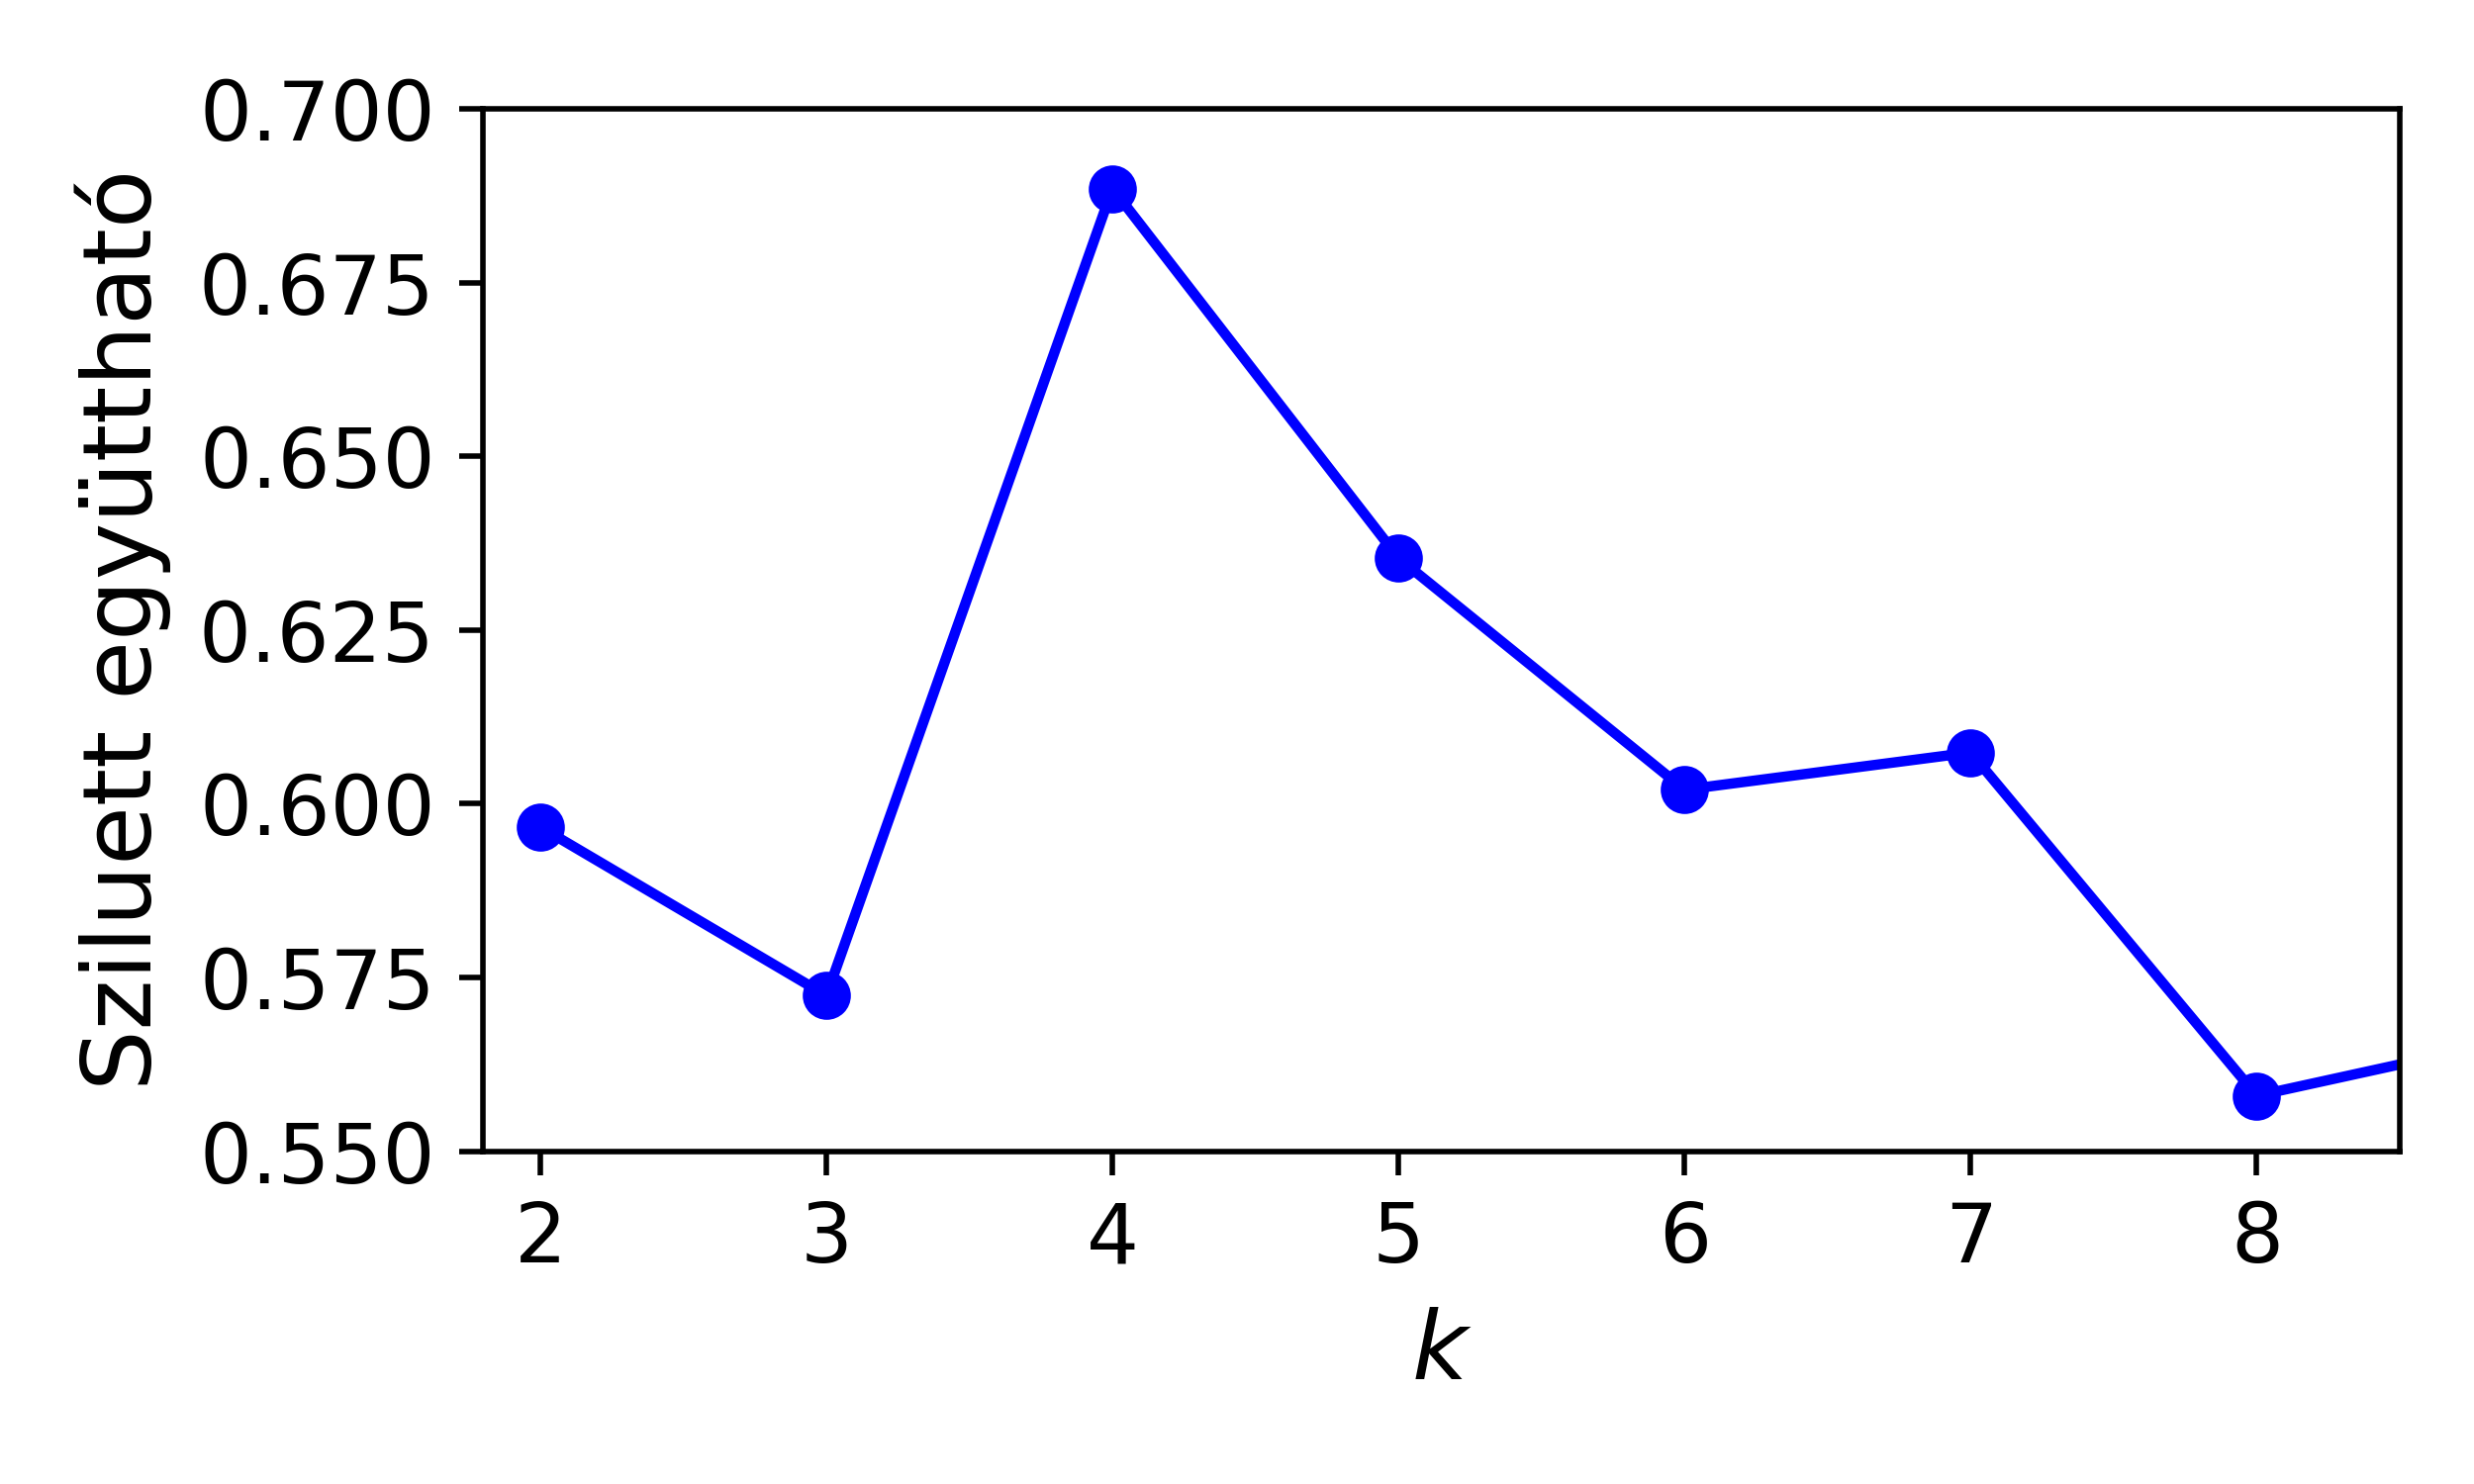
\includegraphics[width=7cm, height=7cm, keepaspectratio]{images/unsupervised_31.png}
\end{center}
A sziluett tartománya: $s\left( i \right) \in \left[ -1, 1 \right]$, ahol:
\vspace{-.3cm}
\begin{itemize}
	\item $-1$: Teljes félreosztályozás
	\item $0$: Közömbös osztályozás
	\item $1$: Tökéletes osztályozás
\end{itemize}
\end{column}
\end{columns}
\end{frame}

\begin{frame}{Teljes konfigurációs tér sziluettje}
\begin{columns}
\begin{column}{.4\textwidth}
A sziluett nem csak mintaegyedekre értelmezhető, hanem terekre is.\par\smallskip
Egy térben helyet foglaló mintaegyedek halmazára vonatkoztatott sziluett-koefficiens a térben megtalálható egyedi pontok sziluettjének átlaga.
\end{column}
\begin{column}{.6\textwidth}
\begin{center}
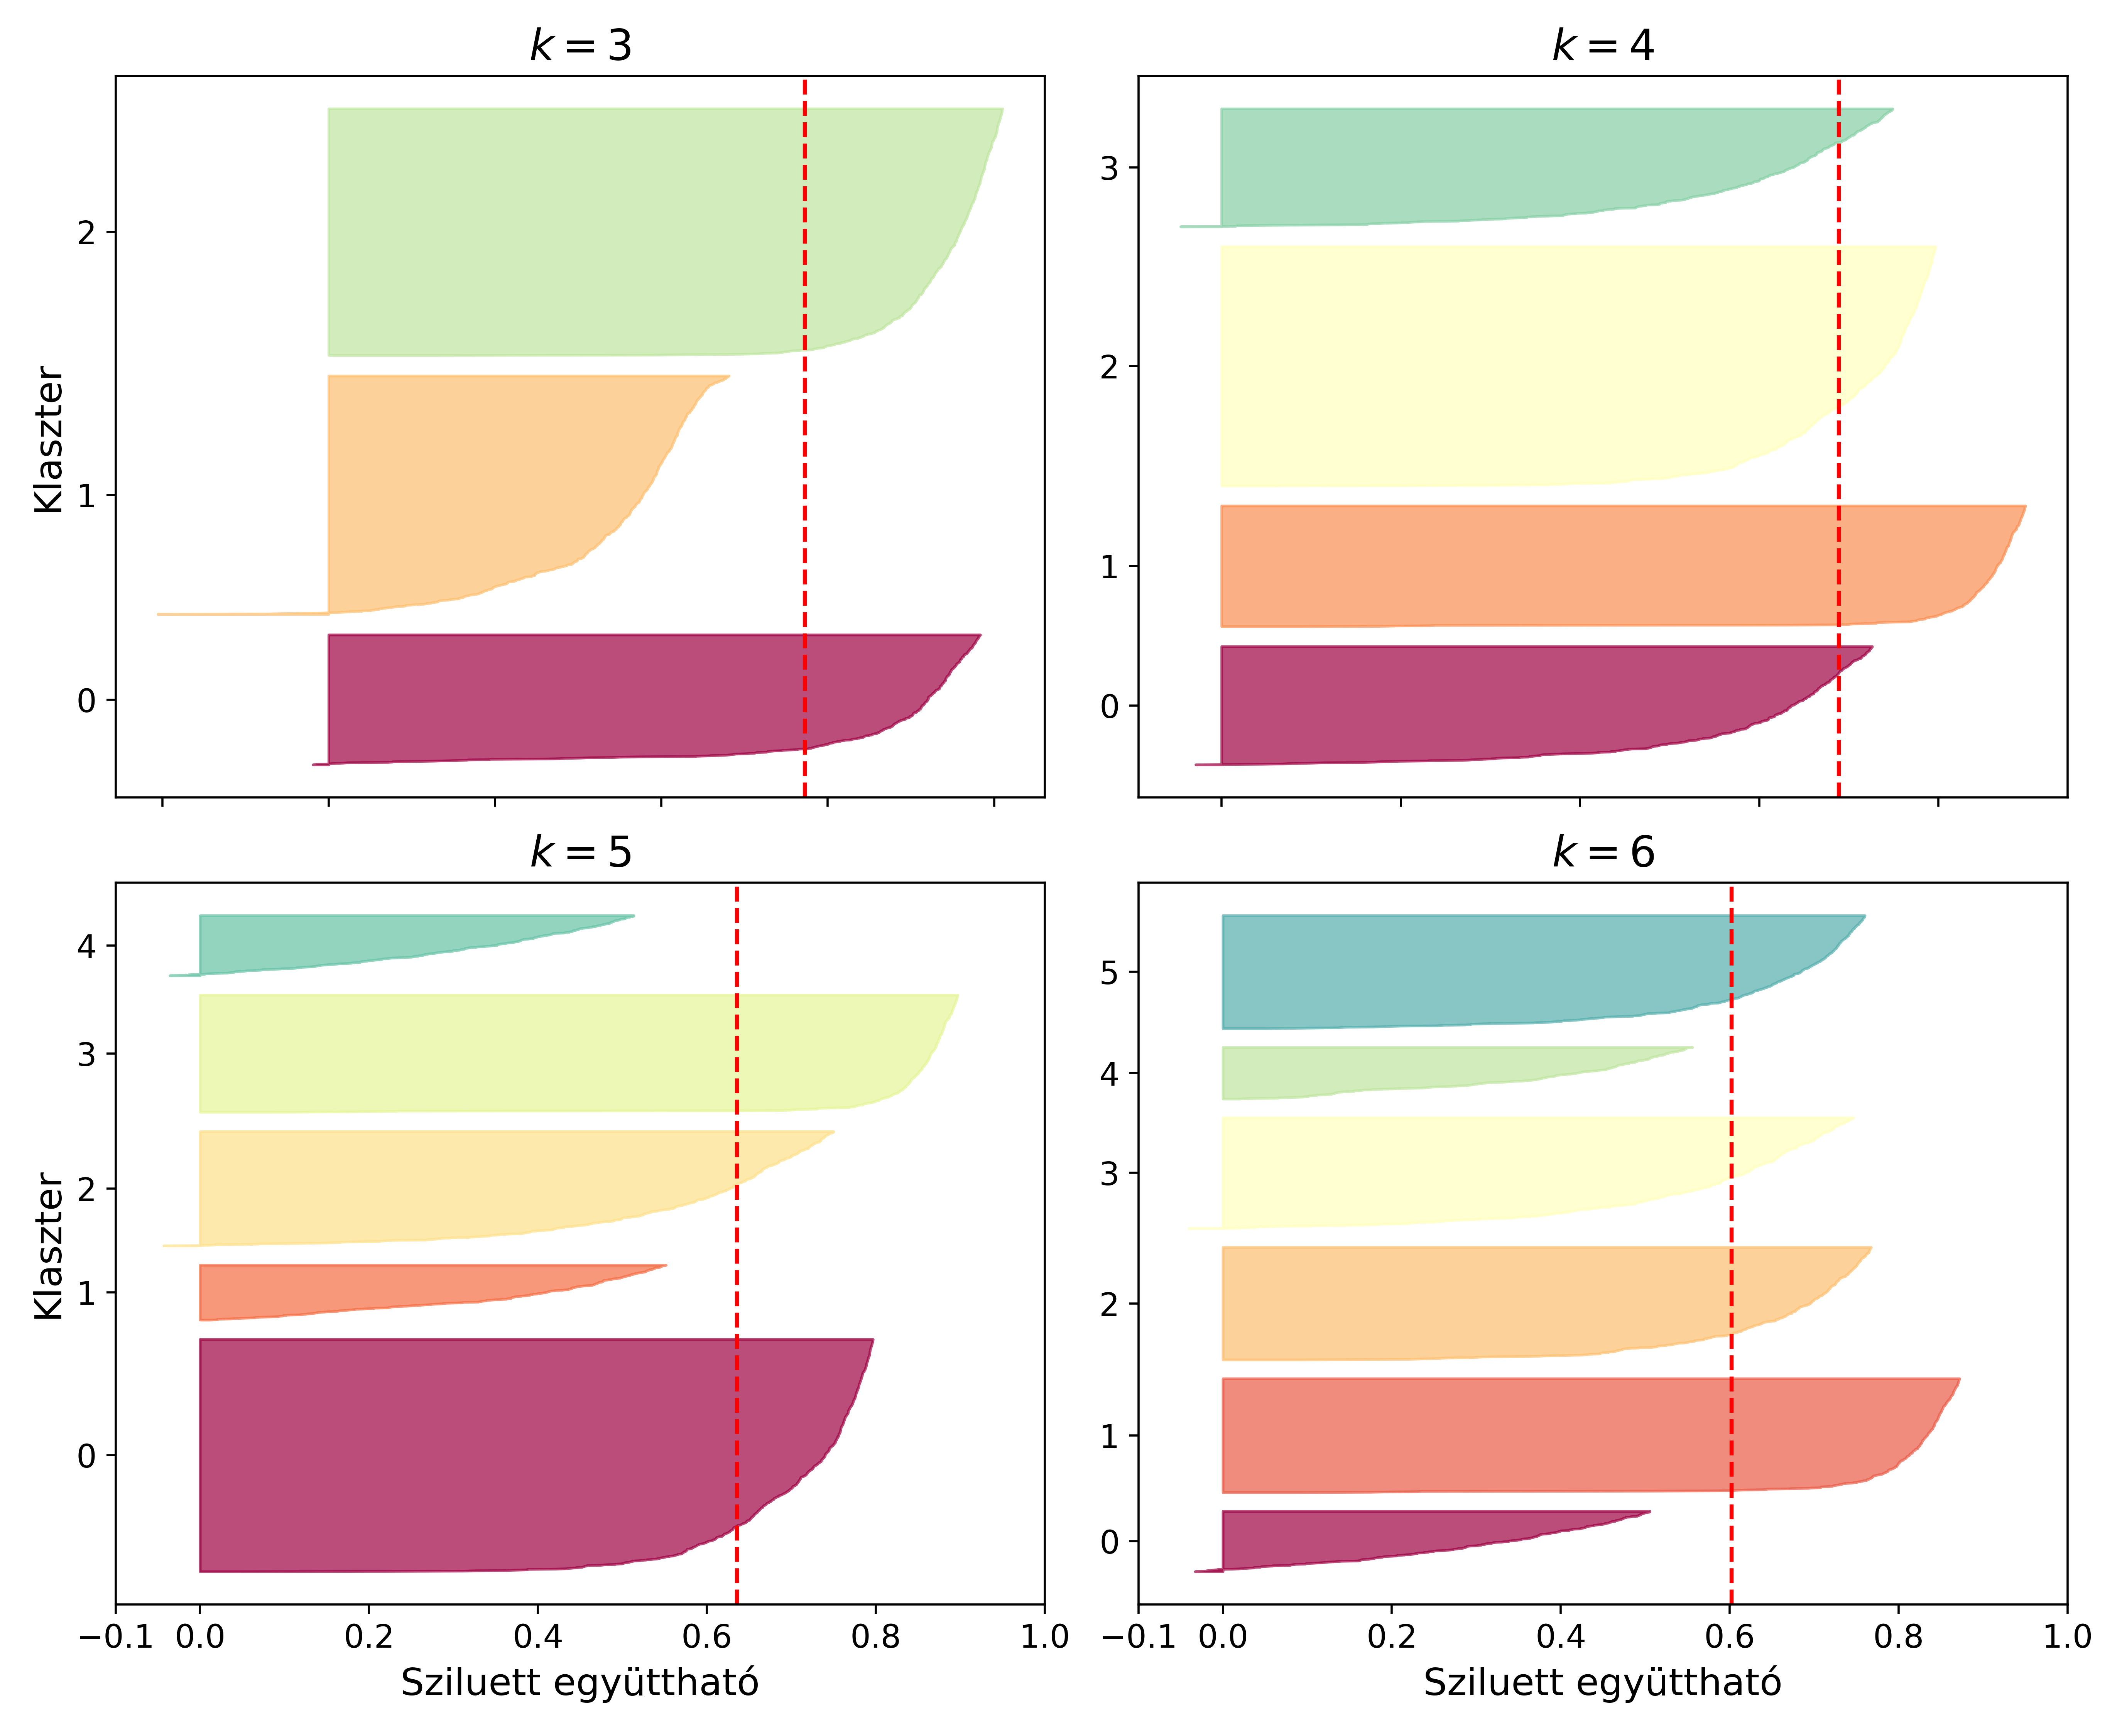
\includegraphics[width=8cm, height=7cm, keepaspectratio]{images/unsupervised_32.png}
\end{center}
\end{column}
\end{columns}
\end{frame}

\begin{frame}{A $K$-közép limitációi}
\begin{columns}
\begin{column}{.5\textwidth}
\only<1-2>{Az algoritmust sokszor kell lefuttatni, hogy a szuboptimális konfigurációkat el lehessen kerülni. A klaszterek számát kézzel kell meghatározni.}
\only<3-4>{A $K$-közép továbbá nem viselkedik megfelelően, amikor a klaszterek méretei és alakjai változatosak, eltérő sűrűségűek. Ez abból ered, hogy a modell két pont távolságát veszi alapul.}
\end{column}
\begin{column}{.5\textwidth}
\begin{center}
\includegraphics<1>[width=7cm, keepaspectratio]{images/unsupervised_28.png}
\includegraphics<2>[width=7cm, keepaspectratio]{images/unsupervised_29.png}
\includegraphics<3>[width=7cm, keepaspectratio]{images/unsupervised_33.png}
\includegraphics<4>[width=7cm, keepaspectratio]{images/unsupervised_34.png}
\end{center}
\end{column}
\end{columns}
\end{frame}

\section{DBSCAN}

\begin{frame}
\tableofcontents[currentsection]
\end{frame}

\begin{frame}{DBSCAN}
\begin{columns}
\begin{column}{.6\textwidth}
A DBSCAN egy sűrűség alapú klaszterezési algoritmus, amely már irreguláris alakzatú klasztereket is képes megbecsülni:
\begin{small}
\begin{enumerate}
	\item Minden egyedhez tartozóan kiszámolja, hány egyed található az $\varepsilon$ sugarú környezetében ($\varepsilon$ szomszédság)
	\item Ha \texttt{min\_samples} küszöbnyi egyed egy $\varepsilon$ szomszédságban, a pontból mag-egyed válik
	\item Minden mintaegyed, amely egy mag-egyed szomszédságában van, a mag-egyed klaszterébe tartozik
	\item A szomszédos mag-egyedek és azok szomszédságai egy klaszterbe tartoznak
	\item Minden mintaegyed, ami nincs egy szomszédságában sem, anomáliának számít
\end{enumerate}
\end{small}
\end{column}
\begin{column}{.4\textwidth}
\begin{center}
\includegraphics<1>[width=6cm, keepaspectratio]{images/unsupervised_37.png}
\includegraphics<2>[width=6cm, keepaspectratio]{images/unsupervised_38.png}
\end{center}
\end{column}
\end{columns}
\end{frame}

\begin{frame}{Predikció DBSCAN modellel}
\begin{columns}
\begin{column}{.5\textwidth}
Meglepő módon a DBSCAN implementációnak nincs \texttt{predict()} metódusa, ezért \textbf{nem tudja egy új egyedről eldönteni, melyik klaszterhez tartozik}.\par\smallskip
Ennek az a mögöttes racionalitása, hogy a DBScan által felismert klasztereken kellően egyszerű futtatni egy osztályozó algoritmust, mint a \texttt{KNeighborsClassifier}. Így képes új egyedeket osztályozni.
\end{column}
\begin{column}{.5\textwidth}
\begin{center}
\includegraphics<1>[width=6cm, height=7cm, keepaspectratio]{images/unsupervised_37.png}
\includegraphics<1>[width=6cm, height=7cm, keepaspectratio]{images/unsupervised_40.png}
\includegraphics<2>[width=6cm, height=7cm, keepaspectratio]{images/unsupervised_38.png}
\includegraphics<2>[width=6cm, height=7cm, keepaspectratio]{images/unsupervised_39.png}
\end{center}
\end{column}
\end{columns}
\end{frame}

\end{document}
























